\documentclass[12pt, oneside]{article} 
\usepackage{amsmath, amsthm, amssymb, calrsfs, wasysym, verbatim, bbm, xcolor, graphicx, fancyhdr, multirow, titlesec, tabularx, spreadtab, pgf-pie, array, longtable, caption, float, subcaption, listings, eso-pic}
\usepackage[a4paper, margin=1cm]{geometry} % modifica le dimensioni della pagina e i margini
\usepackage[italian]{babel}
\usepackage{enumitem}
\usepackage{hyperref}
\hypersetup{breaklinks=true}
% Styling for the Code Snippets
\lstdefinelanguage{JavaScript}{
  morekeywords=[1]{break, continue, delete, else, for, function, if, in,
    new, return, this, typeof, var, void, while, with},
  % Literals, primitive types, and reference types.
  morekeywords=[2]{false, null, true, boolean, number, undefined,
    Array, Boolean, Date, Math, Number, String, Object},
  % Built-ins.
  morekeywords=[3]{eval, parseInt, parseFloat, escape, unescape},
  sensitive,
  morecomment=[s]{/*}{*/},
  morecomment=[l]//,
  morecomment=[s]{/**}{*/}, % JavaDoc style comments
  morestring=[b]',
  morestring=[b]"
}[keywords, comments, strings]

\lstalias[]{ES6}[ECMAScript2015]{JavaScript}

\lstdefinelanguage[ECMAScript2015]{JavaScript}[]{JavaScript}{
  morekeywords=[1]{await, async, case, catch, class, const, default, do,
    enum, export, extends, finally, from, implements, import, instanceof,
    let, static, super, switch, throw, try},
  morestring=[b]` % Interpolation strings.
}

\definecolor{mediumgray}{rgb}{0.3, 0.4, 0.4}
\definecolor{mediumblue}{rgb}{0.0, 0.0, 0.8}
\definecolor{forestgreen}{rgb}{0.13, 0.55, 0.13}
\definecolor{darkviolet}{rgb}{0.58, 0.0, 0.83}
\definecolor{royalblue}{rgb}{0.25, 0.41, 0.88}
\definecolor{crimson}{rgb}{0.86, 0.8, 0.24}

\lstdefinestyle{JSES6Base}{
  backgroundcolor=\color{white},
  basicstyle=\ttfamily,
  breakatwhitespace=false,
  breaklines=true,
  captionpos=b,
  columns=fullflexible,
  commentstyle=\color{mediumgray}\upshape,
  emph={},
  emphstyle=\color{crimson},
  extendedchars=true,  % requires inputenc
  fontadjust=true,
  frame=single,
  identifierstyle=\color{black},
  keepspaces=true,
  keywordstyle=\color{mediumblue},
  keywordstyle={[2]\color{darkviolet}},
  keywordstyle={[3]\color{royalblue}},
  numbers=left,
  numbersep=5pt,
  numberstyle=\tiny\color{black},
  rulecolor=\color{black},
  showlines=true,
  showspaces=false,
  showstringspaces=false,
  showtabs=false,
  stringstyle=\color{forestgreen},
  tabsize=2,
  title=\lstname,
  upquote=true,
}

\definecolor{comment}{rgb}{0.0, 0.5, 0.0}
\definecolor{keyword}{rgb}{0.0, 0.0, 0.75}
\definecolor{string}{rgb}{0.5, 0.0, 0.0}

\lstdefinestyle{typescript}{
    language=JavaScript,
    basicstyle=\ttfamily\footnotesize,
    keywordstyle=\color{keyword}\bfseries,
    stringstyle=\color{string},
    commentstyle=\color{comment}\itshape,
    morekeywords={type, interface, public, private, protected, implements, export, from, as, constructor, readonly},
    literate={=>}{{\(\Rightarrow\)}}{1}
}

\lstdefinestyle{JavaScript}{
  language=JavaScript,
  style=JSES6Base
}
\lstdefinestyle{ES6}{
  language=ES6,
  style=JSES6Base
}
\usepackage{xcolor}

\lstdefinestyle{bashstyle}{
  backgroundcolor=\color{lightgray},
  basicstyle=\ttfamily,
  keywordstyle=\color{blue},
  commentstyle=\color{gray},
  stringstyle=\color{red},
  showstringspaces=false,
  breaklines=true,
  frame=single
}

\lstset{
    basicstyle=\ttfamily,
    keywordstyle=\color{blue},
    commentstyle=\color{green},
    stringstyle=\color{red},
    showstringspaces=false,
    language=bash, % Imposta il linguaggio di default su bash
    frame=single, % Aggiunge un bordo attorno al codice
    framerule=0.5pt, % Spessore del bordo
    breaklines=true, % Permette la divisione delle linee lunghe
    backgroundcolor=\color{lightgray!20}, % Sfondo grigio chiaro
    aboveskip=10pt, % Spazio aggiunto sopra il blocco di codice
    belowskip=10pt  % Spazio aggiunto sotto il blocco di codice
}

\titleclass{\subsubsubsection}{straight}[\subsection]

\newcounter{subsubsubsection}[subsubsection]
\renewcommand\thesubsubsubsection{\thesubsubsection.\arabic{subsubsubsection}}
\renewcommand\theparagraph{\thesubsubsubsection.\arabic{paragraph}} % optional; useful if paragraphs are to be numbered

\titleformat{\subsubsubsection}
  {\normalfont\normalsize\bfseries}{\thesubsubsubsection}{1em}{}
\titlespacing*{\subsubsubsection}
{0pt}{3.25ex plus 1ex minus .2ex}{1.5ex plus .2ex}

\makeatletter
\renewcommand\paragraph{\@startsection{paragraph}{5}{\z@}%
  {3.25ex \@plus1ex \@minus.2ex}%
  {-1em}%
  {\normalfont\normalsize\bfseries}}
\renewcommand\subparagraph{\@startsection{subparagraph}{6}{\parindent}%
  {3.25ex \@plus1ex \@minus .2ex}%
  {-1em}%
  {\normalfont\normalsize\bfseries}}
\def\toclevel@subsubsubsection{4}
\def\toclevel@paragraph{5}
\def\toclevel@paragraph{6}
\def\l@subsubsubsection{\@dottedtocline{4}{7em}{4em}}
\def\l@paragraph{\@dottedtocline{5}{10em}{5em}}
\def\l@subparagraph{\@dottedtocline{6}{14em}{6em}}
\makeatother

\setcounter{secnumdepth}{4}
\setcounter{tocdepth}{4}

\geometry{tmargin=.75in, bmargin=.75in, lmargin=.75in, rmargin = .75in}

\author{RAMtastic6}

%Intestazione
\pagestyle{fancy}
\fancyhf{}
\fancyhead[R]{Gruppo 14 RAMtastic6\\ramtastic6@gmail.com}
\fancyfoot[C]{\thepage}

% Linea intestazione
\renewcommand{\headrulewidth}{1pt} 

% Intestazione documento
\begin{document}
% Salta la prima pagina per l'intestazione
\thispagestyle{empty}
\title{Specifica Tecnica}
\date{29 maggio 2024}
\maketitle
\begin{figure}[h]
  \centering
  
\includegraphics[scale=0.3]{logo.png}
\end{figure}
\begin{center}
    email: ramtastic6@gmail.com
\end{center}

% Informazioni sul documento
\section*{Informazioni sul documento} 
\begin{tabular}{ll}
Versione: & 1.0.0 \\
Redattori: &  Zaupa R. Visentin S. Brotto D. Basso L. Tonietto F. Zambon M. \\
Verificatori: & Brotto D. Visentin S. Zambon M. Zaupa R. Tonietto F. \\
Destinatari: & Vardanega T., Cardin R., Imola Informatica \\
Uso: & Esterno
\end{tabular}
\newpage

% Registro dei cambiamenti
\section*{Registro dei Cambiamenti - Changelog}
\begin{longtable}{|c|c|c|c|p{7cm}|}
\hline
\textbf{Versione} & \textbf{Data} & \textbf{Autore} & \textbf{Verificatore} & 
\textbf{Dettaglio} \\
\hline
v 1.0.0 & 2024-05-29 & Brotto D. & Brotto D. & Approvazione e validazione del documento \\
\hline
v 0.5.0 & 2024-05-28 & Visentin S. & Tonietto F. & Modificata $\textit{architettura}_G$ $\textit{websocket}_G$ e aggiunta sezione database  \\
\hline
v 0.4.6 & 2024-05-28 & Brotto D. & Tonietto F. & Specificato modulo staff; aggiunti diagrammi $\textit{UML}_G$ (con descrizioni) di craete\_reservation, user, admin e notifications  \\
\hline
v 0.4.5 & 2024-05-28 & Zambon M. & Tonietto F. & Aggiunto e descritto l'$\textit{UML}_G$ del sign-up-admin  \\
\hline
v 0.4.4 & 2024-05-27 & Zaupa R. & Tonietto F. & Descritto il modulo Notification del $\textit{backend}_G$ e sistemato lo stato dei requisiti funzionali \\
\hline
v 0.4.3 & 2024-05-26 & Zambon M. & Zaupa R. & Descritto il $\textit{Backend}_G$ for $\textit{Frontend}_G$ pattern, il Compound Components pattern e il Controlled inputs pattern (sezione 4.2.2) \\
\hline
v 0.4.2 & 2024-05-26 & Visentin S. & Zaupa R. & Modificato il diagramma delle classi del $\textit{backend}_G$ \\
\hline
v 0.4.1 & 2024-05-26 & Zambon M. & Zaupa R. & Aggiunti gli endpoints per User (sezione 4.1.1) \\
\hline
v 0.4.0 & 2024-05-25 & Visentin S. & Zambon M. & Aggiunti gli endpoints per Restaurant, Reservation, Orders e Food (sezione 4.1.1) \\
\hline
v 0.3.3 & 2024-05-25 & Tonietto F. & Zambon M. & Aggiunta la descrizione del Publisher-Subscriber pattern relativa al Websocket (4.2.3.1) \\
\hline
v 0.3.2 & 2024-05-25 & Basso L. & Zambon M. & Aggiornata la sezione requisiti; inserite le sezioni riguardati i moduli back-end Authentication, Menu, DaysOpen; inserito diagramma $\textit{UML}_G$ del server socket (sezione 4.1.3); inseriti $\textit{UML}_G$ pagina order e order checkout (sezione 4.1.2.5) con relativa descrizione. \\
\hline
v 0.3.1 & 2024-05-25 & Visentin S. & Zambon M. & Stesura del Module pattern (sezione 4.2.1.5) \\
\hline
v 0.3.0 & 2024-05-24 & Tonietto F. & Zambon M. & Aggiunto l'$\textit{UML}_G$ del Login ($\textit{frontend}_G$). \\
\hline
v 0.2.2 & 2024-05-24 & Visentin S. & Zambon M. & Continuata la stesura della sezione 3.3, aggiuniti $\textit{Repository}_G$ pattern e Controller-Service pattern \\
\hline
v 0.2.1 & 2024-05-24 & Visentin S. & Zambon M. & Aggiunta sezione 3.3 (Esecuzione dei $\textit{test}_G$), dependy injection e decorator pattern\\
\hline
v 0.2.0 & 2024-05-23 & Tonietto F. & Visentin S. & Aggiunte le motivazioni relative alla scelta di Socket.io come libreria per l'implementazione del Websocket (2.1.6). Aggiunto l'uso di un pacchetto per scrivere frammenti di codice. \\
\hline
v 0.1.4 & 2024-05-22 & Zaupa R. & Visentin S. & Soddisfatti ROF12 ROF13 ROF14 ROF19 ROF30 ROF31 ROF34\\
\hline
v 0.1.3 & 2024-05-22 & Brotto D. & Visentin S. & Soddisfatto ROF57 \\
\hline
v 0.1.2 & 2024-05-13 & Basso L. & Visentin S. & Aggiunta alla sezione 4 il diagramma del $\textit{sistema}_G$ di notifica. \\
\hline
v 0.1.1 & 2024-05-13 & Brotto D. & Visentin S. & Aggiunta sezione 3 \\
\hline
v 0.1.0 & 2024-05-13 & Visentin S. & Brotto D. & Aggiungo schema ER del database \\
\hline
v 0.0.3 & 2024-05-13 & Zaupa R. & Brotto D. & Prima stesura della sezione "Stato dei requisiti funzionali" e della sottosezione "$\textit{Architettura}_G$ di $\textit{deployment}_G$"\\
\hline
v 0.0.2 & 2024-05-07 & Zaupa R. & Brotto D. & Prima stesura della sezione "$\textit{Tecnologie}_G$"\\
\hline
v 0.0.1 & 2024-05-04 & Zaupa R. & Brotto D. & Prima versione, stesura della sezione "Introduzione" \\
\hline
\end{longtable}
\newpage

% Sommario
\tableofcontents
\newpage

% Introduzione
\section{Introduzione}
\subsection{Scopo del documento}
Il presente documento si propone di definire le metriche e le metodologie di controllo e misurazione necessarie per garantire la qualità del prodotto e del processo. In particolare, le metriche di valutazione del prodotto sono correlate ai requisiti e alle aspettative del fornitore.
Il Piano di Qualifica è concepito per essere dinamico ed incrementale, in particolar modo per quanto riguarda le metriche descritte e mira a fornire una valutazione il più obiettiva possibile di ciò che è stato realizzato.\\
Le procedure del Way of Working devono essere costantemente osservate e migliorate, al fine di garantire che il prodotto soddisfi le aspettative del cliente e mantenga gli standard di qualità richiesti. Eventuali termini tecnici sono definiti all'interno del documento "Glossario Tecnico".

\subsection{Riferimenti}
\subsubsection{Riferimenti normativi}
\begin{enumerate}
    \item Norme di Progetto
    \item Presentazione del capitolato d'appalto C3 - Progetto Easy Meal: \\ 
    \url{https://www.math.unipd.it/~tullio/IS-1/2023/Progetto/C3.pdf}
    \item Regolamento del progetto didattico: \\ 
    \url{https://www.math.unipd.it/~tullio/IS-1/2023/Dispense/PD2.pdf}
\end{enumerate}
\subsubsection{Riferimenti informativi}
\label{sec:rif_inf}
\begin{enumerate}
    \item Lezione \emph{"Progettazione software (T6)"} del corso di Ingegneria del software: \\
    \url{https://www.math.unipd.it/~tullio/IS-1/2023/Dispense/T6.pdf}
    \item Lezione \emph{"Qualità del software (T7)"} del corso di Ingegneria del software: \\
    \url{https://www.math.unipd.it/~tullio/IS-1/2023/Dispense/T7.pdf}
    \item Lezione \emph{"Qualità di processo (T8)"} del corso di Ingegneria del software: \\
    \url{https://www.math.unipd.it/~tullio/IS-1/2023/Dispense/T8.pdf}
    \item Lezione \emph{"Verifica e validazione: introduzione (T9)"} del corso di Ingegneria del software: \\
    \url{https://www.math.unipd.it/~tullio/IS-1/2023/Dispense/T9.pdf}
    \item Lezione \emph{"Verifica e validazione: analisi statica (T10)"} del corso di Ingegneria del software: \\
    \url{https://www.math.unipd.it/~tullio/IS-1/2023/Dispense/T10.pdf}
    \item Lezione \emph{"Verifica e validazione: analisi dinamica (T11)"} del corso di Ingegneria del software: \\
    \url{https://www.math.unipd.it/~tullio/IS-1/2023/Dispense/T11.pdf}
     \item Documento \emph{"Dichiarazione impegni v1.2"}: \\ \url{https://github.com/RAMtastic6/Project14/blob/main/documenti/CANDIDATURA/documento_impegni_v1.2.pdf}
     \item Metriche di progetto (\emph{Earned Value Analysis}):\\
     \url{https://it.wikipedia.org/wiki/Metriche_di_progetto}
\end{enumerate}
\subsection{Codifica delle metriche}
In questa sottosezione verranno definite le metriche che utilizzeremo, utilizzando un codice standardizzato.

Una metrica è identificata dal seguente formato di codice:
\[
\text{M[Tipo][Id]-[Acronimo]}
\]

Dove:
\begin{itemize}
    \item \textbf{M} sta per "Metrica"
    \item \textbf{Tipo} può essere PC (per un processo) o PD (per un prodotto)
    \item \textbf{Id} rappresenta un identificativo all'interno di una metrica di un certo tipo
    \item \textbf{Acronimo} indica l'acronimo del nome della metrica utilizzata
\end{itemize}

Per ciascuna metrica verranno fornite descrizioni, valori accettabili e valori preferibili.
\newpage

% Tecnologie
\section{Tecnologie}
In questa sezione viene presentata una panoramica degli strumenti e delle $\textit{tecnologie}_G$ utilizzate per l'implementazione del $\textit{sistema}_G$ denominato $\textit{Easy Meal}_G$. 
\subsection{Tecnologie implementative}
\subsubsection{Next.js}
Next.js è un $\textit{framework}_G$ di sviluppo per applicazioni basato su $\textit{React}_G$. La sua scelta è stata dettata dalla sua efficienza e dalla sua facilità d'uso. L'utilizzo di tale $\textit{framework}_G$ permette di creare applicazioni veloci e performanti oltre che effettuare il rendering lato server. Offre una supporto integrato per TypeScript, funzionalità avanzate di realizzazione di $\textit{API}_G$, gestione del routing e Server Action.
\begin{itemize}
    \item \textbf{Versione scelta}: 14.0.4
    \item \textbf{Documentazione}: \url{https://nextjs.org/}\\
    (Consultato: 2024-05-13)
    \item \textbf{Linguaggio}: TypeScript, $\textit{JSX}_G$, $\textit{JSON}_G$.
\end{itemize}

\subsubsection{React}
React è una libreria JavaScript utilizzata per la creazione di interfacce utente dinamiche e reattive.
\begin{itemize}
    \item \textbf{Versione scelta:} 18.0.0
    \item \textbf{Documentazione}: \url{https://reactjs.org/}\\
    (Consultato: 2024-05-13)
    \item \textbf{Linguaggio}: TypeScript, $\textit{JSX}_G$, $\textit{JSON}_G$.
\end{itemize}

\subsubsection{Tailwind CSS}
Tailwind $\textit{CSS}_G$ è un $\textit{framework}_G$ $\textit{CSS}_G$ utilizzato per lo sviluppo di interfacce web lato utente offrendo classi predefinite per applicare lo stile agli elementi.
\begin{itemize}
    \item \textbf{Versione scelta:} 3.4.1
    \item \textbf{Documentazione}: \url{https://tailwindcss.com/}\\
    (Consultato: 2024-05-13)
    \item \textbf{Linguaggio}: CSS
\end{itemize}

\subsubsection{Node.js}
Node.js è un $\textit{runtime system}_G$ $\textit{open-source}_G$ orientato agli eventi che esegue codice JavaScript $\textit{server-side}_G$.

\begin{itemize}
    \item \textbf{Versione scelta:} 21.0.0
    \item \textbf{Documentazione}: \url{https://nodejs.org/}\\
    (Consultato: 2024-05-13)
    \item \textbf{Linguaggio}: TypeScript, JSON
\end{itemize}

\subsubsection{Nest.js}
Nest.js è un $\textit{framework}_G$ $\textit{typescript}_G$ basato su $\textit{Node.js}_G$ e progettato per sviluppare applicazioni $\textit{server-side}_G$ efficienti, scalabili e manutenibili. 

\begin{itemize}
    \item \textbf{Versione scelta:} 10.0.0
    \item \textbf{Documentazione}: \url{https://nestjs.com/}\\
    (Consultato: 2024-05-13)
    \item \textbf{Linguaggio}: TypeScript, JSON
\end{itemize}

\subsubsection{Socket.io}
Socket.io è una libreria JavaScript che permette la comunicazione in tempo reale bidirezionale tra client e server tramite $\textit{websocket}_G$, con supporto per la trasmissione di eventi. È progettata per facilitare lo sviluppo di applicazioni web interattive e collaborative, come chat in tempo reale, giochi multiplayer e applicazioni di monitoraggio in tempo reale. \\
In particolare, la scelta di utilizzare Socket.io è stata dettata da vari fattori. Innanzitutto, essendo giunta più in là nello sviluppo la necessità di utilizzare una libreria a parte per la realizzazione di alcuni requisiti obbligatori, ci si è orientati verso una libreria che fosse nativamente supportata dai $\textit{framework}_G$ utilizzati per $\textit{Frontend}_G$ e $\textit{Backend}_G$. Altri aspetti che hanno portato il gruppo a scegliere la sua adozione sono stati l'ampia documentazione e la gestione efficace di connessioni, disconnessioni e riconoscimento degli eventi fornita dalla libreria. 
\begin{itemize}
\item \textbf{Versione scelta:} 4.0.0
\item \textbf{Documentazione}: \url{https://socket.io/docs/v4/}\\
(Consultato: 2024-05-13)
\item \textbf{Linguaggi}: JavaScript, TypeScript
\end{itemize}

\subsection{Tecnologie per la persistenza dei dati}
\subsubsection{PostgreSQL}
PostgreSQL è un $\textit{sistema}_G$ di gestione di database relazionali $\textit{open-source}_G$, noto per la sua affidabilità e robustezza.
\begin{itemize}
\item \textbf{Versione scelta:} 15.2
\item \textbf{Documentazione}: \url{https://www.postgresql.org/}\\
(Consultato: 2024-05-13)
\item \textbf{Linguaggi}: SQL
\end{itemize}

\newpage
\subsection{Tecnologie per il testing}
\subsubsection{Jest}
Jest è un $\textit{framework}_G$ di $\textit{test}_G$ del $\textit{software}_G$ $\textit{open-source}_G$ per JavaScript, sviluppato da Facebook. È progettato per essere semplice da utilizzare e offre un'esperienza di sviluppo fluida e piacevole per i $\textit{test}_G$ unitari, di integrazione e di $\textit{sistema}_G$.
\begin{itemize}
\item \textbf{Versione scelta:} 29.7.0
\item \textbf{Documentazione}: \url{https://jestjs.io/docs/getting-started}\\
(Consultato: 2024-05-13)
\item \textbf{Linguaggi}: TypeScript, JavaScript
\end{itemize}
\subsection{Tecnologie per il deployment}
\subsubsection{Docker}
Docker è un $\textit{software}_G$ utilizzato per effettuare il $\textit{deployment}_G$ di un prodotto $\textit{software}_G$. La sua caratteristica è di permettere la scalabilità e l'Isolamento delle applicazioni utilizzando la virtualizzazione a livello di $\textit{sistema}_G$ operativo. Offre una discreta efficienza, portabilità e facilità d'uso.
\begin{itemize}
    \item \textbf{Versione scelta}: latest
    \item \textbf{Documentazione}: \url{https://www.docker.com/}\\
    (consultato: 2024-05-13)
\end{itemize}
\subsubsection{Docker Compose}
$\textit{Docker}_G$ Compose è uno $\textit{strumento}_G$ per la definizione e l'esecuzione di applicazioni aventi più' container. Permette di gestire i container $\textit{Docker}_G$ semplificando il $\textit{processo}_G$ di $\textit{deployment}_G$.
\begin{itemize}
    \item \textbf{Versione scelta}: latest
    \item \textbf{Documentazione}: \url{https://docs.docker.com/compose/}\\
    (Consultato: 2024-05-13)
\end{itemize}
\newpage

% Esecuzione software
\section{Esecuzione del software}
\subsection{Download del progetto}
Clonare il $\textit{repository}_G$ del progetto usando il comando: 
\begin{lstlisting}[language=bash]
git clone https://github.com/RAMtastic6/EasyMeal.git 
cd EasyMeal
\end{lstlisting}

\subsection{Avvio dell'applicazione} 
\subsubsection{Docker (consigliato)}
Questo progetto utilizza $\textit{Docker}_G$ Compose per gestire l'avvio dei container $\textit{Docker}_G$. 
Per avviare i container e utilizzare l'applicazione si seguando le seguenti istruzioni.

\begin{itemize}
\item \textbf{Avvio dei container} \\
Per avviare i container utilizzando $\textit{Docker}_G$ Compose, esegui il seguente comando nella directory del progetto:
\begin{lstlisting}[language=bash]
docker-compose up --build --watch
\end{lstlisting}

Oppure per far partire i servizi senza che la console di comando attendi la chiusura si usi il comando:
\begin{lstlisting}[language=bash]
docker-compose up -d
\end{lstlisting}

Una volta avviati i container, si potrà accedere all'applicazione utilizzando il browser o gli strumenti di sviluppo appropriati. \\ Per esempio per poter accedere al progetto NextJS ci si colleghi al link: 
\begin{quote}
\begin{verbatim}
http://localhost:3000/create_reservation 
\end{verbatim}
\end{quote}
Si tenga presente che NextJS utilizza la porta 3000, NestJS 6969, Postgres utilizza 7070 e Socket 8000.
\\
\item \textbf{Modifica dei file Dockerfile e compose.yaml} \\
Per applicare le modifiche e far partire il progetto si usi il comando:
\begin{lstlisting}[language=bash]
docker-compose up --build
\end{lstlisting}

\end{itemize}

\newpage
\subsubsection{NPM}
Senza l'utilizzo di $\textit{Docker}_G$ si devono installare manualmente le seguenti $\textit{tecnologie}_G$:
\begin{itemize}
    \item Node.js
    \item $\textit{npm}_G$ (Node Package Manager)
    \item postgresSQL
\end{itemize}
Si ricorda di importare il dump del database nel proprio computer, per farlo si può usare pgAdmin.\\ \\ Ora si eseguano le seguenti istruzioni:
\begin{enumerate}
\item Installare le dipendenze per il $\textit{backend}_G$ $\textit{Nest.js}_G$:
\begin{lstlisting}[language=bash]
cd nest-js
npm install
\end{lstlisting}

\item Avviare il server $\textit{backend}_G$ $\textit{Nest.js}_G$:
\begin{lstlisting}[language=bash]
npm run start:dev
\end{lstlisting}

\item Installare le dipendenze per il $\textit{frontend}_G$ $\textit{Next.js}_G$: Aprire una nuova shell lasciando la precedente in esecuzione
\begin{lstlisting}[language=bash]
cd next-js
npm install
\end{lstlisting}

\item Avviare il server $\textit{frontend}_G$ $\textit{Next.js}_G$:
\begin{lstlisting}[language=bash]
npm run dev
\end{lstlisting}

\item Installare le dipendenze per il progetto socket $\textit{Nest.js}_G$:
\begin{lstlisting}[language=bash]
cd websocket-server
npm install
\end{lstlisting}

\item Avviare il server socket $\textit{Nest.js}_G$:
\begin{lstlisting}[language=bash]
npm run start:dev
\end{lstlisting}

\item Accedere all'applicazione:
Una volta avviati sia il server $\textit{backend}_G$ $\textit{Nest.js}_G$ che il server $\textit{frontend}_G$ $\textit{Next.js}_G$, è possibile accedere all'applicazione utilizzando il browser. \\ Si apra il browser e si vada all'indirizzo 
\begin{quote}
\begin{verbatim}
    $\textit{http}_G$://localhost:3000/create_reservation
\end{verbatim}
\end{quote}
per accedere alla pagina di creazione delle prenotazioni.

\end{enumerate}

\subsection{Esecuzione dei test}
In questa sezione si elencano i comandi per eseguire i $\textit{test}_G$ tramite $\textit{jest}_G$ per tutti i servizi.
Per poter eseguire i $\textit{test}_G$ in locale per i tre servizi si dovrà prima installare $\textit{Node.js}_G$ versione 21.x . \href{https://nodejs.org/en/download/package-manager/current}{$\textit{Node.js}_G$ installazione}(consultato: 2024-05-27) \\
I comandi per eseguire i $\textit{test}_G$ dei vari servizi sono gli stessi, si deve solo cambiare la cartella dove vengono eseguiti i comandi:
\begin{itemize}
\item Per i $\textit{test}_G$ lato $\textit{backend}_G$:
\begin{lstlisting}[language=bash]
cd nest-js
\end{lstlisting}
\item Per i $\textit{test}_G$ lato $\textit{frontend}_G$:
\begin{lstlisting}[language=bash]
cd next-js
\end{lstlisting}
\item Per i $\textit{test}_G$ del $\textit{websocket}_G$:
\begin{lstlisting}[language=bash]
cd websocket-server
\end{lstlisting}
\end{itemize}
Quindi, di seguito, vengono riportati i comandi per eseguire i $\textit{test}_G$:
\begin{enumerate}
\item Eseguire il comando, se non fatto in precedenza:
\begin{lstlisting}[language=bash]
npm install
\end{lstlisting}
\item Eseguire il seguente script per l'esecuzione di tutti i $\textit{test}_G$ generando un report finale:
\begin{lstlisting}[language=bash]
npm run $\textit{test}_G$:cov
\end{lstlisting}
\item Aprire il seguente file per visualizzare il report:
\begin{lstlisting}[language=bash]
./coverage/coverage.txt
\end{lstlisting}
\end{enumerate}
\newpage

% Architettura
\section{Architettura}
\begin{comment}
\subsection{Architettura di sistema}
\end{comment}
\subsection{Architettura logica}
Il progetto EasyMeal è strutturato in tre componenti principali:
\begin{itemize}
\item \textbf{Backend}: Responsabile della gestione della $\textit{logica di business}_G$ e della persistenza dei dati. Il $\textit{backend}_G$ si occupa di stabilire e mantenere la connessione con il database, nonché di fornire i mezzi per salvare e accedere ai dati.
\item \textbf{Frontend}: Destinato alla presentazione dei dati ottenuti dal $\textit{backend}_G$, il $\textit{frontend}_G$ consente all'utente di interagire con le funzionalità del progetto in modo intuitivo e user-friendly.
\item \textbf{WebSocket Server}: Abilita la comunicazione in tempo reale tra i diversi client del $\textit{frontend}_G$, permettendo l'aggiornamento istantaneo dei dati e migliorando l'interattività dell'applicazione.
\end{itemize}
\subsubsection{Backend}
Nel $\textit{backend}_G$ si è scelto di utilizzare il $\textit{framework}_G$ NestJS, che permette la realizzazione di un servizio $\textit{API}_G$ REST. L'$\textit{architettura}_G$ del $\textit{backend}_G$ è suddivisa nei seguenti strati:
\begin{itemize}
\item \textbf{Controller Layer}: Si occupa del routing delle richieste. I controller fungono da intermediari tra il client e i servizi, gestendo la presentation layer e instradando le richieste del client ai servizi appropriati.
\item \textbf{Service Layer}: Gestisce la $\textit{logica di business}_G$ dell'applicazione. Questo strato è responsabile delle operazioni e delle regole di business, garantendo che tutte le operazioni siano eseguite correttamente.
\item \textbf{Data Access Layer}: Implementato tramite $\textit{TypeORM}_G$ (Object-Relational Mapping) che facilita l'interazione con il database realizzato tramite PostegreSQL. Questo strato gestisce la persistenza dei dati, fornendo i mezzi per salvare, recuperare e manipolare i dati nel database.
\end{itemize}
L'adozione di NestJS e la suddivisione in questi strati facilitano lo sviluppo, la $\textit{manutenzione}_G$ e la scalabilità del $\textit{backend}_G$ del progetto EasyMeal, conformandosi all'$\textit{architettura}_G$ \textbf{multi-tier} a 3-tier.\\
\newline
Di seguito viene riportato il diagramma $\textit{UML}_G$ del $\textit{backend}_G$.
\begin{figure}[H]
    \centering
    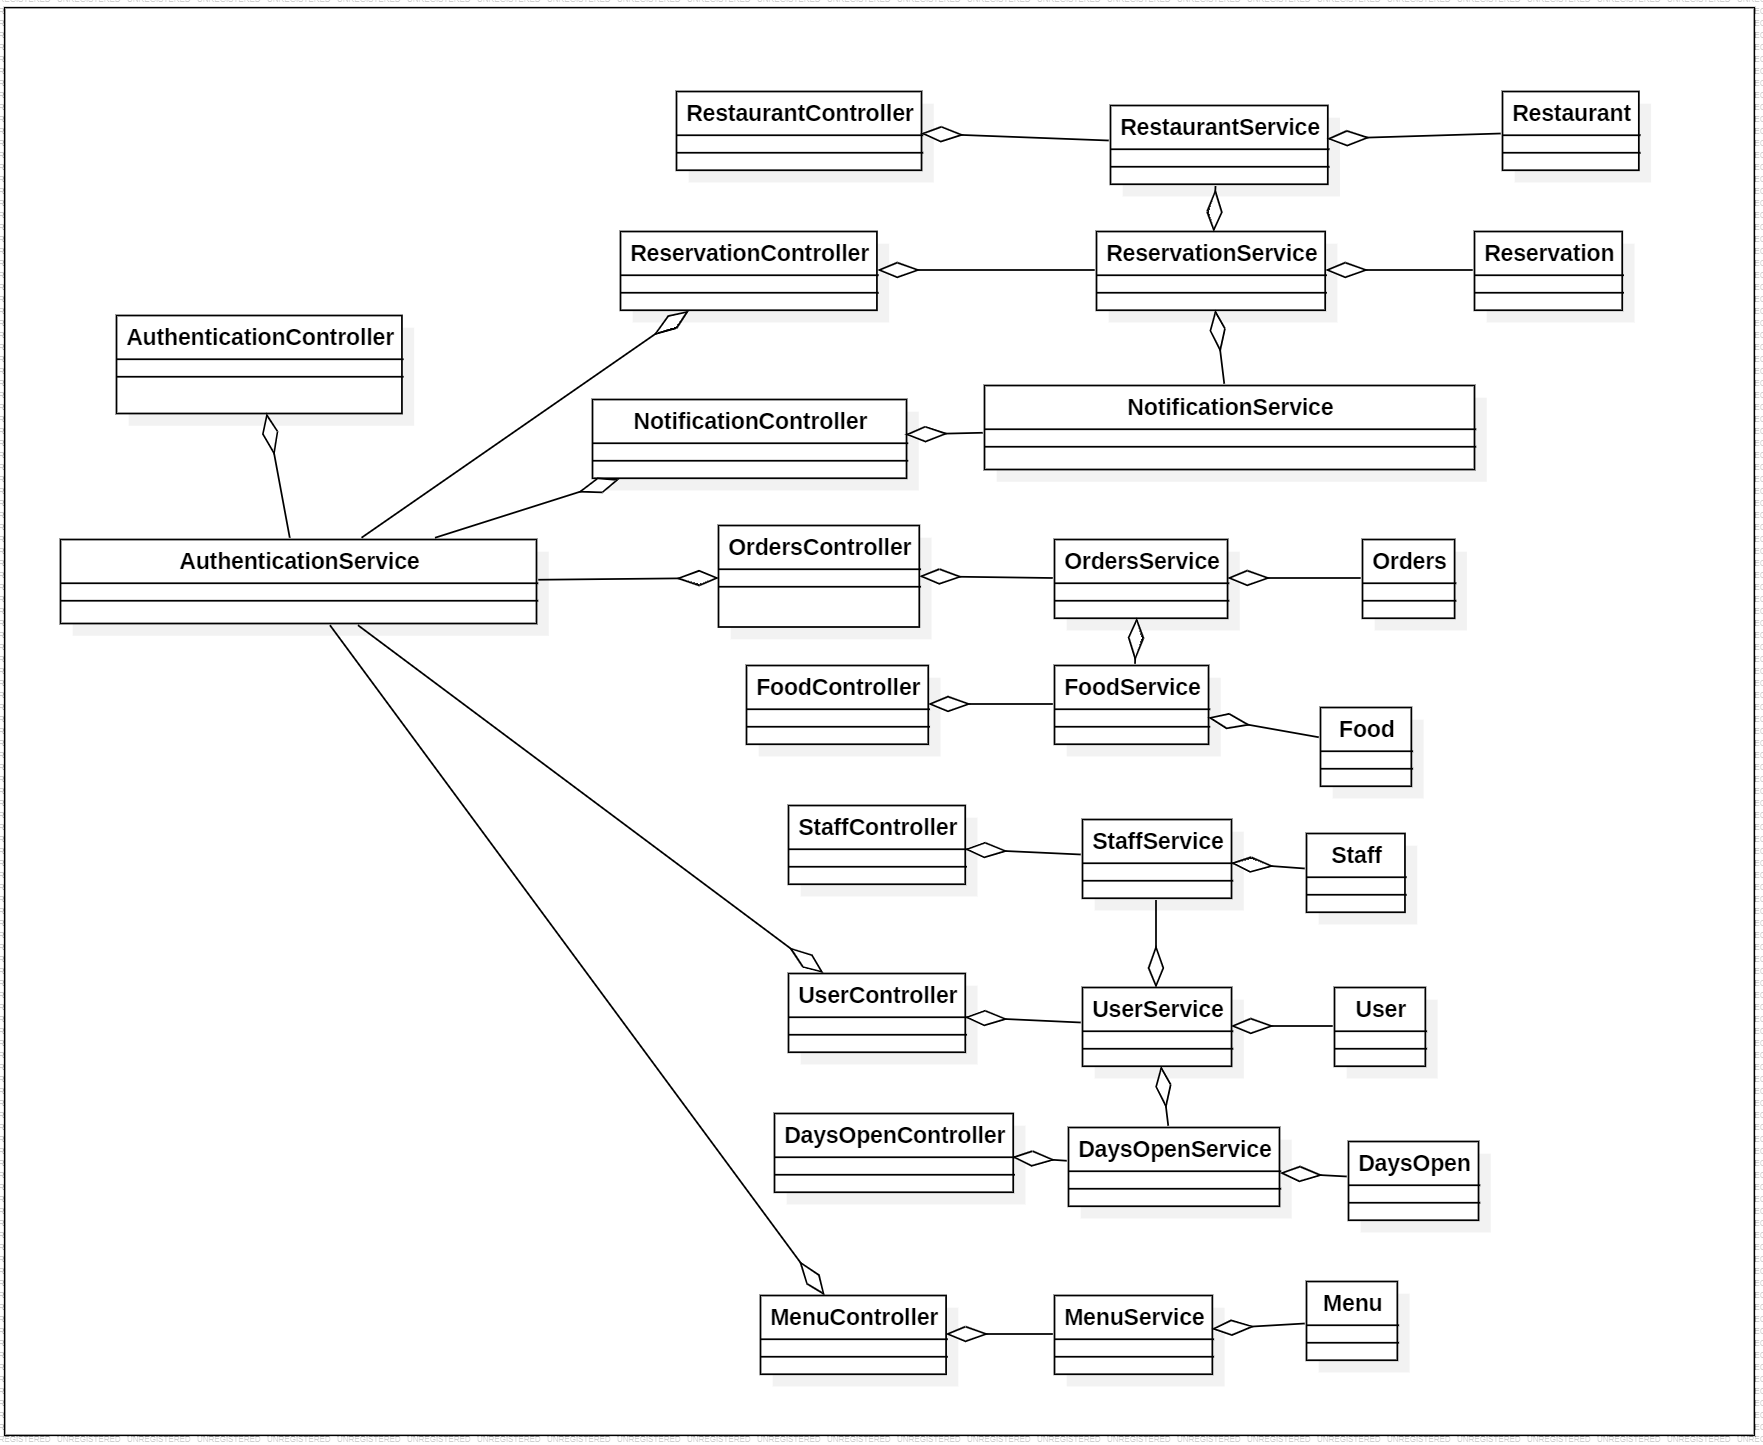
\includegraphics[width=\linewidth]{images/backenduml.png}
    \caption{Diagramma delle classi del backend}
    \label{fig:schemaER}
\end{figure}
Di seguito si elencano le $\textit{api}_G$ fornite dal $\textit{backend}_G$ raggruppate per moduli:
\subsubsubsection{Authentication}
\paragraph{signin}

\begin{itemize}
    \item \textbf{Endpoint}: /authentication/signin
    \item \textbf{Metodo}: POST
    \item \textbf{Parametri}: AuthenticationDTO
    \item \textbf{Descrizione}: questa funzione si occupa di prendere in input email e password; nel caso in cui le credenziali siano valide e già presenti all'interno del $\textit{sistema}_G$, viene generato un token in formato $\textit{JWT}_G$ e ritornato; in caso contrario viene lanciata un'$\textit{eccezione}_G$.
\end{itemize}

\paragraph{decodeToken}: 

\begin{itemize}
    \item \textbf{Endpoint}: /authentication/decodeToken
    \item \textbf{Metodo}: POST
    \item \textbf{Parametri}: DecodeTokenDTO
    \item \textbf{Descrizione}: la funzione prende in input una stringa in formato $\textit{JWT}_G$; nel caso la stringa non dovesse rispettare il formato, viene lanciata un'$\textit{eccezione}_G$; in caso contrario, viene verificata la validità del token all'interno del $\textit{sistema}_G$; nel caso in cui il token sia valido, viene ritornato un oggetto, il quale rappresenta l'id dell'utente e il ruolo di quest'ultimo all'interno del $\textit{sistema}_G$.
\end{itemize}

\subsubsubsection{Daysopen}

\paragraph{create}
\begin{itemize}
    \item \textbf{Endpoint}: /daysopen
    \item \textbf{Metodo}: POST
    \item \textbf{Parametri}: CreateDaysOpenDTO
    \item \textbf{Descrizione}: la funzione permette di creare un elenco di giorni di apertura associati ad un determinato ristorante se presente all'interno del $\textit{sistema}_G$.
\end{itemize}

\subsubsubsection{Food}
\paragraph{findOne}:
\begin{itemize}
    \item \textbf{Endpoint}: /food/:id
    \item \textbf{Metodo}: GET
    \item \textbf{Parametri}: id: number
    \item \textbf{Descrizione}: questa funzione ritorna il piatto, con i relativi ingredienti, associato all'id.
\end{itemize}
\subsubsubsection{Menu}
\paragraph{create} 

\begin{itemize}
    \item \textbf{Endpoint}: /menu
    \item \textbf{Metodo}: POST
    \item \textbf{Parametri}: CreateMenuDto
    \item \textbf{Descrizione}: la funzione crea un menù (lista di piatti) associato ad un ristorante presente all'interno del $\textit{sistema}_G$.
\end{itemize}

\subsubsubsection{Notification}
\paragraph{create}:
\begin{itemize}
    \item \textbf{Metodo}: POST
    \item \textbf{Parametri}: NotificationDto
    \item \textbf{Descrizione}: la funzione crea una notifica utilizzando un oggetto NotificationDto. Innanzitutto viene salvato un oggetto notification nel database, poi viene inviata una notifica al $\textit{websocket}_G$ effettuando una richiesta POST all'url \url{http://socket:8000/notification/send}. Infine, viene restituito il messaggio del risultato dell'operazione di salvataggio della notifica. 
\end{itemize}
\paragraph{findAllByUserId}:

\begin{itemize}
    \item \textbf{Endpoint}: /notification
    \item \textbf{Metodo}: POST
    \item \textbf{Parametri}: FindAllByUserIdDTO
    \item \textbf{Descrizione}: la funzione cerca tutte le notifiche corrispondenti a un determinato ID utente e restituisce un array di oggetti notifica contenenti le proprietà \emph{id}, \emph{title}, \emph{message} e \emph{status}.
\end{itemize}
\paragraph{updateStatus}:
\begin{itemize}
    \item \textbf{Endpoint}: /notification/update
    \item \textbf{Metodo}: POST
    \item \textbf{Parametri}: updateStatusDTO
    \item \textbf{Descrizione}: la funzione aggiorna lo stato di una notifica specificata tramite l'id. In breve, viene ricercata nel database una notifica corrispondente all'id fornito e se non viene trovata viene restituito null. Se la notifica viene trovata, viene impostato lo stato della notifica come \emph{READ}. Infine, la notifica aggiornata viene salvata nel database e viene restituita. 
\end{itemize}
\paragraph{findOne}:
\begin{itemize}
    \item \textbf{Metodo}: POST
    \item \textbf{Parametri}: id
    \item \textbf{Descrizione}: la funzione restituisce la notifica trovata nel database corrispondente all'id fornito.
\end{itemize}
\subsubsubsection{Orders}
\paragraph{create}:
\begin{itemize}
    \item \textbf{Endpoint}: /orders
    \item \textbf{Metodo}: POST
    \item \textbf{Parametri}: reservation\_id: number, food\_id: number, token: string
    \item \textbf{Descrizione}: questa funzione salva nel database una nuova $\textit{ordinazione}_G$ associata alla $\textit{prenotazione}_G$ con id uguale a reservation\_id.
\end{itemize}
\paragraph{findAll}:
\begin{itemize}
    \item \textbf{Endpoint}: /orders
    \item \textbf{Metodo}: GET
    \item \textbf{Descrizione}: questa funzione ritorna tutti gli ordini presenti nel database.
\end{itemize}
\paragraph{findOne}:
\begin{itemize}
    \item \textbf{Endpoint}: /orders/findOne
    \item \textbf{Metodo}: POST
    \item \textbf{Parametri}: FindOneDTO
    \item \textbf{Descrizione}: questa funzione ritorna la $\textit{ordinazione}_G$ con l'id corrispondente.
\end{itemize}
\paragraph{addQuantity}:
\begin{itemize}
    \item \textbf{Endpoint}: /orders/addQuantity
    \item \textbf{Metodo}: POST
    \item \textbf{Parametri}: AddQuantityDTO
    \item \textbf{Descrizione}: la funzione salva nel database la quantità del piatto appartenente all'$\textit{ordinazione}_G$ appropriata.
\end{itemize}
\paragraph{updateIngredients}:
\begin{itemize}
    \item \textbf{Endpoint}: /orders/updateIngredients
    \item \textbf{Metodo}: POST
    \item \textbf{Parametri}: UpdateIngredientsDTO
    \item \textbf{Descrizione}: questa funzione aggiorna la lista degli ingredienti associati alla $\textit{ordinazione}_G$.
\end{itemize}
\paragraph{remove}:
\begin{itemize}
    \item \textbf{Endpoint}: /orders/remove
    \item \textbf{Metodo}: POST
    \item \textbf{Parametri}: RemoveDTO
    \item \textbf{Descrizione}: questa funzione rimuove dal database l'$\textit{ordinazione}_G$ dalla $\textit{prenotazione}_G$ appropriata.
\end{itemize}
\paragraph{partialBill}:
\begin{itemize}
    \item \textbf{Endpoint}: /orders/partialBill
    \item \textbf{Metodo}: POST
    \item \textbf{Parametri}: PartialBillDTO
    \item \textbf{Descrizione}: questa funzione ritorna quanto un utente deve pagare col metodo "paga la tua parte".
\end{itemize}
\paragraph{romanBill}:
\begin{itemize}
    \item \textbf{Endpoint}: /orders/romanBill
    \item \textbf{Metodo}: POST
    \item \textbf{Parametri}: RomanBillDTO
    \item \textbf{Descrizione}: questa funzione ritorna quanto un utente deve pagare col metodo "pagamento alla romana".
\end{itemize}
\paragraph{totalBill}:
\begin{itemize}
    \item \textbf{Endpoint}: /orders/totalBill
    \item \textbf{Metodo}: POST
    \item \textbf{Parametri}: reservation\_id: number
    \item \textbf{Descrizione}: questa funzione ritorna il totale da pagare di una $\textit{prenotazione}_G$ con id associato.
\end{itemize}
\paragraph{checkOrdersPayStatus}:
\begin{itemize}
    \item \textbf{Endpoint}: /orders/checkOrdersPayStatus
    \item \textbf{Metodo}: POST
    \item \textbf{Parametri}: token: string, reservation\_id
    \item \textbf{Descrizione}: questa funzione ritorna true se tutte le ordinazioni di un utente associate ad una $\textit{prenotazione}_G$ sono state pagate, altrimenti ritorna \emph{false}.
\end{itemize}
\paragraph{updateListOrders}:
\begin{itemize}
    \item \textbf{Endpoint}: /orders/updateListOrders
    \item \textbf{Metodo}: POST
    \item \textbf{Parametri}: UpdateListOrders
    \item \textbf{Descrizione}: questa funzione salva nel database la lista degli ingredienti delle ordinazioni di una $\textit{prenotazione}_G$, confermando le ordinazioni.
\end{itemize}
\subsubsubsection{Reservation}
\paragraph{create}:
\begin{itemize}
    \item \textbf{Endpoint}: /reservation
    \item \textbf{Metodo}: POST
    \item \textbf{Parametri}: CreateReservationDto
    \item \textbf{Descrizione}: la funzione, attraverso i dati in input deve creare una nuova $\textit{prenotazione}_G$, verificando che il ristorante non sia già pieno nel giorno della $\textit{prenotazione}_G$, successivamente salvando nel database la nuova $\textit{prenotazione}_G$ se avvenuta con successo.
\end{itemize}
\paragraph{addCustomer}:
\begin{itemize}
    \item \textbf{Endpoint}: /reservation/addCustomer
    \item \textbf{Metodo}: POST
    \item \textbf{Parametri}: AddCustomerDto
    \item \textbf{Descrizione}: questa funzione aggiunge, dopo la verifica del token, un utente ad una $\textit{prenotazione}_G$ già creata in precedenza se ha ancora posti disponibili.
\end{itemize}
\paragraph{findAll}:
\begin{itemize}
    \item \textbf{Endpoint}: /reservation/
    \item \textbf{Metodo}: GET
    \item \textbf{Descrizione}: questa funzione restituisce la lista di tutte le prenotazioni
\end{itemize}
\paragraph{findOne}:
\begin{itemize}
    \item \textbf{Endpoint}: /reservation/:id
    \item \textbf{Metodo}: GET
    \item \textbf{Parametri}: id: number
    \item \textbf{Descrizione}: questa funzione ritorna la $\textit{prenotazione}_G$ con l'id desiderato, oppure ritorna not found se non trovato.
\end{itemize}
\paragraph{getMenuWithOrdersQuantityByReservationId}:
\begin{itemize}
    \item \textbf{Endpoint}: /reservation/:id/orders
    \item \textbf{Metodo}: GET
    \item \textbf{Parametri}: id: number
    \item \textbf{Descrizione}: questa funzione ritorna il menu con la quantità degli ordini già effettuati della $\textit{prenotazione}_G$ con id specificato.
\end{itemize}
\paragraph{getReservationsByRestaurantId}:
\begin{itemize}
    \item \textbf{Endpoint}: /reservation/restaurant/:restaurantId
    \item \textbf{Metodo}: GET
    \item \textbf{Parametri}: id: number
    \item \textbf{Descrizione}: questa funzione ritorna tutte le prenotazioni associate all'id del ristorante
\end{itemize}
\paragraph{getReservationsByUserId}:
\begin{itemize}
    \item \textbf{Endpoint}: /reservation/user/:userId
    \item \textbf{Metodo}: GET
    \item \textbf{Parametri}: id: number
    \item \textbf{Descrizione}: questa funzione ritorna tutte le $\textit{prenotazione}_G$ associate all'user id.
\end{itemize}
\paragraph{verifyReservation}:
\begin{itemize}
    \item \textbf{Endpoint}: /reservation/verify
    \item \textbf{Metodo}: POST
    \item \textbf{Parametri}: verifyReservationDto
    \item \textbf{Descrizione}: questa funzione controlla, attraverso il token passato in input, se lo user appartiene ad una $\textit{prenotazione}_G$.
\end{itemize}
\paragraph{getReservationByAdminId}:
\begin{itemize}
    \item \textbf{Endpoint}: /reservation/admin
    \item \textbf{Metodo}: POST
    \item \textbf{Parametri}: ReservationAdminDTO
    \item \textbf{Descrizione}: questa funzione ritorna tutte le prenotazioni del ristorante associato all'admin (amministratore del ristorante).
\end{itemize}
\paragraph{getUserOfReservation}:
\begin{itemize}
    \item \textbf{Endpoint}: /reservation/:id/user\_token
    \item \textbf{Metodo}: POST
    \item \textbf{Parametri}: id: number, token: string
    \item \textbf{Descrizione}: questa funzione ritorna la $\textit{prenotazione}_G$ con l'id desiderato se anche l'utente associato al token ne fa parte.
\end{itemize}
\paragraph{acceptReservation}:
\begin{itemize}
    \item \textbf{Endpoint}: /reservation/:id/accept
    \item \textbf{Metodo}: POST
    \item \textbf{Parametri}: id: number
    \item \textbf{Descrizione}: questa funzione salva nel database lo stato "accepted" nella $\textit{prenotazione}_G$ con id appropriato.
\end{itemize}
\paragraph{rejectReservation}:
\begin{itemize}
    \item \textbf{Endpoint}: /reservation/:id/reject
    \item \textbf{Metodo}: POST
    \item \textbf{Parametri}: id: number
    \item \textbf{Descrizione}: questa funzione salva nel database lo stato "rejected" nella $\textit{prenotazione}_G$ con id appropriato.
\end{itemize}
\paragraph{completeReservation}:
\begin{itemize}
    \item \textbf{Endpoint}: /reservation/:id/complete
    \item \textbf{Metodo}: POST
    \item \textbf{Parametri}: id: number
    \item \textbf{Descrizione}: questa funzione salva nel database lo stato "compleated" nella $\textit{prenotazione}_G$ con id appropriato.
\end{itemize}
\paragraph{setPaymentMethod}:
\begin{itemize}
    \item \textbf{Endpoint}: /reservation/setPaymentMethod
    \item \textbf{Metodo}: POST
    \item \textbf{Parametri}: token: string, reservation\_id: number, isRomanBill: boolean 
    \item \textbf{Descrizione}: questa funzione salva nel database il metodo di pagamento della $\textit{prenotazione}_G$ associata a reservation\_id, il token viene utilizzato per verificare l'utente.
\end{itemize}
\subsubsubsection{Restaurant}
\paragraph{getFilteredRestaurants}:
\begin{itemize}
    \item \textbf{Endpoint}: /restaurant/filter
    \item \textbf{Metodo}: GET
    \item \textbf{Parametri}: query, currentPage: number, items\_per\_pege: number,
    \item \textbf{Descrizione}: questa funzione ritorna la lista dei ristoranti filtrati per nome, data, città e tipologia cucina
\end{itemize}
\paragraph{create}:
\begin{itemize}
    \item \textbf{Endpoint}: /restaurant
    \item \textbf{Metodo}: POST
    \item \textbf{Parametri}: RestaurantDTO
    \item \textbf{Descrizione}: questa funzione salva nel database un nuovo ristorante con i parametri in input.
\end{itemize}
\paragraph{findAll}:
\begin{itemize}
    \item \textbf{Endpoint}: /restaurant
    \item \textbf{Metodo}: GET
    \item \textbf{Descrizione}: questa funzione ritorna la lista di tutti i ristoranti presenti nel database.
\end{itemize}
\paragraph{findAllCuisines}:
\begin{itemize}
    \item \textbf{Endpoint}: /restaurant/cuisines
    \item \textbf{Metodo}: GET
    \item \textbf{Descrizione}: questa funzione ritorna tutte le tipologie di cucine presenti nel database.
\end{itemize}
\paragraph{findAllCities}:
\begin{itemize}
    \item \textbf{Endpoint}: /restaurant/cities
    \item \textbf{Metodo}: GET
    \item \textbf{Descrizione}: questa funzione ritorna la lista di tutte le città dei ristoranti prensenti nel database.
\end{itemize}
\paragraph{getNumberOfFilteredRestaurants}:
\begin{itemize}
    \item \textbf{Endpoint}: /restaurant/count
    \item \textbf{Metodo}: GET
    \item \textbf{Parametri}: query
    \item \textbf{Descrizione}: questa funzione ritorna il numero dei ristoranti disponibili con i filtri passati in input, ovvero: città, nome, data e tipologia cucina.
\end{itemize}
\paragraph{findOne}:
\begin{itemize}
    \item \textbf{Endpoint}: /restaurant/:id
    \item \textbf{Metodo}: GET
    \item \textbf{Parametri}: id: number
    \item \textbf{Descrizione}: questa funzione ritorna il ristorante con l'id associato.
\end{itemize}
\paragraph{getBookedTables}:
\begin{itemize}
    \item \textbf{Endpoint}: /restaurant/:id/booked-tables
    \item \textbf{Metodo}: GET
    \item \textbf{Parametri}: id: number, date: string
    \item \textbf{Descrizione}: questa funzione ritorna il numero di prenotazioni di un ristorante in un determinato giorno.
\end{itemize}
\paragraph{getRestaurantAndMenuByRestaurantId}:
\begin{itemize}
    \item \textbf{Endpoint}: /restaurant/filter
    \item \textbf{Metodo}: GET
    \item \textbf{Parametri}: id: number
    \item \textbf{Descrizione}: questa funzione ritorna il nuovo membro dello staff associato all'id con le informazioni del menu.
\end{itemize}

\subsubsubsection{Staff}
\paragraph{create}:
\begin{itemize}
    \item \textbf{Endpoint}: /staff
    \item \textbf{Metodo}: POST
    \item \textbf{Parametri}: StaffDto
    \item \textbf{Descrizione}: questa funzione salva nel database un nuovo membro dello staff con i parametri in input.
\end{itemize}
\paragraph{getRestaurantIdByAdminId}:
\begin{itemize}
    \item \textbf{Endpoint}: /staff/:id/restaurant
    \item \textbf{Metodo}: GET 
    \item \textbf{Parametri}: restaurant\_id: number
    \item \textbf{Descrizione}: questa funzione ritorna il ristorante associato all’admin (ovvero l'amministratore del ristorante).
\end{itemize}

\subsubsubsection{User}
\paragraph{create}:
\begin{itemize}
    \item \textbf{Endpoint}: /user/user
    \item \textbf{Metodo}: POST
    \item \textbf{Parametri}: UserDto
    \item \textbf{Descrizione}: questa funzione, attraverso i dati di input , crea un nuovo utente verificando che l'email dell'utente non sia già presente nel database.
\end{itemize}
\paragraph{createAdmin}:
\begin{itemize}
    \item \textbf{Endpoint}: /user/admin
    \item \textbf{Metodo}: POST
    \item \textbf{Parametri}: AdminDto
    \item \textbf{Descrizione}: questa funzione, attraverso i dati di input , crea un nuovo utente admin verificando che l'utente e il ristorante non siano già presenti nel database.
\end{itemize}
\paragraph{findOne}:
\begin{itemize}
    \item \textbf{Endpoint}: /user/:id
    \item \textbf{Metodo}: GET
    \item \textbf{Parametri}: id: number
    \item \textbf{Descrizione}: questa funzione ritorna l'utente con l'id desiderato, oppure ritorna not found se non trovato.
\end{itemize}
\begin{comment}
\paragraph{findUserByEmail}:
\begin{itemize}
    \item \textbf{Parametri}: email: string
    \item \textbf{Descrizione}: questa funzione ritorna l'utente con l'email inserita, oppure ritorna not found se non trovato
\end{itemize}
\paragraph{create\_user\_manager}:
\begin{itemize}
    \item \textbf{Parametri}: UserDto, manager: EntityManager
    \item \textbf{Descrizione}: questa funzione, attraverso i dati di input , deve creare un nuovo utente manager, verificando che non sia già presente nel database; successivamente il nuovo utente manager viene salvato nel database, se la creazione è avvenuta con successo.
\end{itemize}
\end{comment}
\newpage
\subsubsection{Frontend}
Per il $\textit{frontend}_G$, è stato utilizzato $\textit{Next.js}_G$, un $\textit{framework}_G$ basato su $\textit{React}_G$. Questa scelta ha portato all'adozione della $\textit{React}_G$ Architecture, che si basa sulla suddivisione della logica in vari componenti. Ogni componente gestisce una parte specifica della logica dell'applicazione, permettendo di creare pagine web utilizzando questi componenti.
Inoltre, $\textit{Next.js}_G$ supporta la \textit{Server-Side Rendering} ($\textit{SSR}_G$), che consente al server del $\textit{frontend}_G$ di renderizzare le pagine prima di restituirle al client. Questo migliora le prestazioni iniziali del caricamento delle pagine e ottimizza l'indicizzazione sui motori di ricerca.
La struttura delle cartelle del progetto $\textit{frontend}_G$ è organizzata come segue:
\begin{verbatim}
src
 |- actions
 |- app
 |- components
\end{verbatim}
Dove:
\begin{itemize}
\item \textbf{src}: È la cartella root del progetto $\textit{Next.js}_G$.
\item \textbf{actions}: Contiene tutte le Server Actions, che sono responsabili della gestione delle operazioni lato server, come il fetching dei dati e altre logiche $\textit{server-side}_G$.
\item \textbf{app}: Contiene le pagine renderizzate lato server ($\textit{SSR}_G$), che vengono generate dal server e inviate al client.
\item \textbf{components}: Contiene i componenti lato client, che gestiscono la logica e l'interfaccia utente sul lato client.
\end{itemize}
Questa $\textit{architettura}_G$ offre diversi vantaggi:
\begin{itemize}
\item \textbf{Riutilizzabilità}: I componenti, essendo progettati per gestire logiche specifiche, possono essere facilmente riutilizzati in diverse parti dell'applicazione. Questo riduce la duplicazione del codice e facilita la $\textit{manutenzione}_G$.
\item \textbf{Manutenibilità}: La suddivisione in componenti rende il codice più organizzato e modulare. Ogni componente può essere sviluppato, testato e mantenuto in modo indipendente.
\item \textbf{Composizione}: Le pagine vengono costruite componendo diversi componenti, rendendo semplice la costruzione di interfacce complesse a partire da parti più semplici e gestibili.
\end{itemize}
Per illustrare meglio l'$\textit{architettura}_G$ adottata, vengono riportati i diagrammi delle classi per le pagine principali. Questi diagrammi mostrano come i componenti sono strutturati e come interagiscono tra loro per formare l'interfaccia utente.
In sintesi, l'uso di $\textit{Next.js}_G$ e della $\textit{React}_G$ Architecture ha permesso di creare un $\textit{frontend}_G$ modulare, riutilizzabile e facilmente mantenibile, migliorando l'efficienza dello sviluppo e la qualità del codice.
\subsubsubsection{Admin}
\begin{figure}[H]
    \centering
    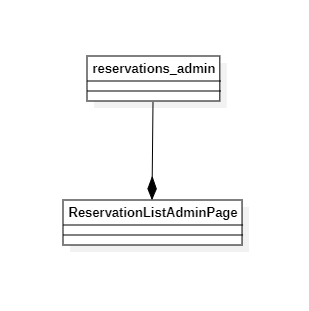
\includegraphics[width=0.4\linewidth]{images/reservationS_admin_page.png}
    \caption{Diagramma UML pagina della lista prenotazione - Admin}
    \label{fig:restaurant_page}
\end{figure}
\paragraph{Descrizione} La pagina della lista prenotazioni per l'admin riporta tutte le prenotazioni che sono state fatte per il suo ristorante. Di ogni $\textit{prenotazione}_G$ nella lista si visualizzano: id, numero di partecipanti, data, ora, un bottone per accedere alla singola $\textit{prenotazione}_G$ e lo stato attuale in cui si trova la $\textit{prenotazione}_G$ (in attesa di conferma, da pagare, accettata, rifiutata, e completata).


\begin{figure}[H]
    \centering
    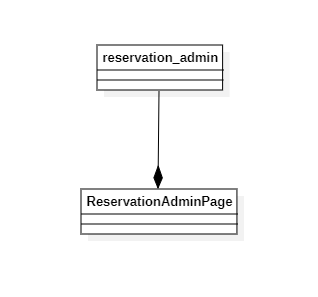
\includegraphics[width=0.4\linewidth]{images/reservation_admin_page.png}
    \caption{Diagramma UML pagina della singola prenotazione - Admin}
    \label{fig:restaurant_page}
\end{figure}
\paragraph{Descrizione} La pagina della singola $\textit{prenotazione}_G$ permette all'admin di visualizzare i dati della $\textit{prenotazione}_G$ con la possibilità di:
\begin{itemize}
    \item  accettare o rifiutare una nuova richiesta di $\textit{prenotazione}_G$;
    \item  visualizzare i pasti ordinati se la $\textit{prenotazione}_G$ è stata accettata o completata;
    \item  visualizzare il costo totale e/o parziale se lo ordinazioni sono state confermate.
\end{itemize}



\subsubsubsection{Create\_reservation}
\begin{figure}[H]
    \centering
    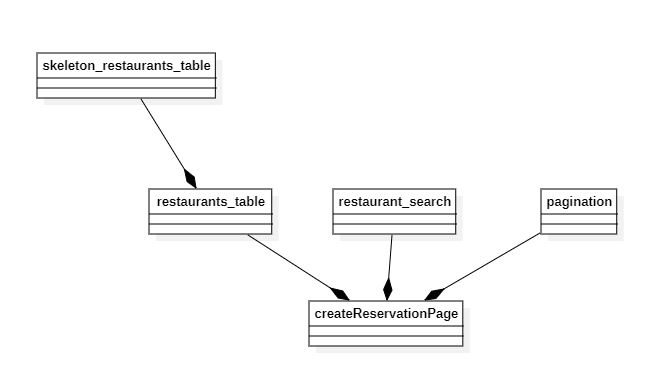
\includegraphics[width=0.8\linewidth]{images/create_reservation_page.png}
    \caption{Diagramma UML pagina di prenotazione}
    \label{fig:create_reservation_page}
\end{figure}
\paragraph{Descrizione} La pagina della $\textit{prenotazione}_G$ permette all'utente di cercare un ristorante dove vuole effettuare una $\textit{prenotazione}_G$, basandosi su nome, città, cucina e data. 
La ricerca tramite questi filtri permette di visualizzare i ristoranti che li soddisfano per poi procedere con la $\textit{prenotazione}_G$ vera e propria.


\begin{figure}[H]
    \centering
    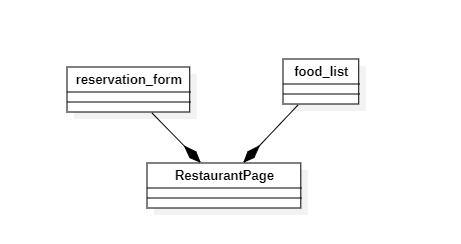
\includegraphics[width=0.6\linewidth]{images/restaurant_page.png}
    \caption{Diagramma UML pagina del ristorante}
    \label{fig:restaurant_page}
\end{figure}
\paragraph{Descrizione} La pagina del ristorante, dopo che è stato scelto il ristorante dalla lista di quelli presenti, permette di visualizzare diversi dati del ristorante scelto, tra cui indirizzo, città, cucina e il menù.
Sempre nella stessa pagina vi è un form per la finalizzazione della $\textit{prenotazione}_G$, in cui sono richiesti i dati: data, orario di arrivo e numero di partecipanti. Inseriti questi dati si può richiedere di effettuare una $\textit{prenotazione}_G$, dopodiché l'utente verrà reindirizzata alla pagina reservation user.


\subsubsubsection{Login}
\begin{figure}[H]
    \centering
    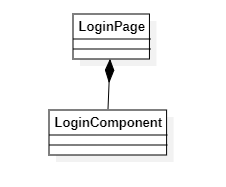
\includegraphics[width=0.3\linewidth]{images/login.png}
    \caption{Diagramma UML Login}
    \label{fig:UML-login}
\end{figure}
\paragraph{Descrizione} La pagina login permette all'utente di inserire la propria email e password e accedere al sito se le credenziali corrispondono ad un account. Se il login ha successo l'utente sarà reindirizzato alla pagina create reservation. 

\subsubsubsection{Notifications}
\begin{figure}[H]
    \centering
    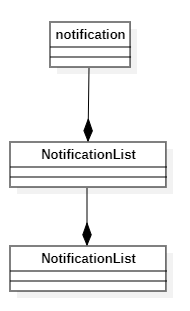
\includegraphics[width=0.3\linewidth]{images/notification_page.png}
    \caption{Diagramma UML pagina notifiche}
    \label{fig:UML-notification_page}
\end{figure}
\paragraph{Descrizione} La pagina della lista delle notifiche permette di visualizzare la lista di tutte le notifiche ricevute in merito allo stato di una $\textit{prenotazione}_G$ incluso il pagamento. La pagina è utilizzata sia per l'amministratore del ristorante che per l'utente base.

\subsubsubsection{Order}
\begin{figure}[H]
    \centering
    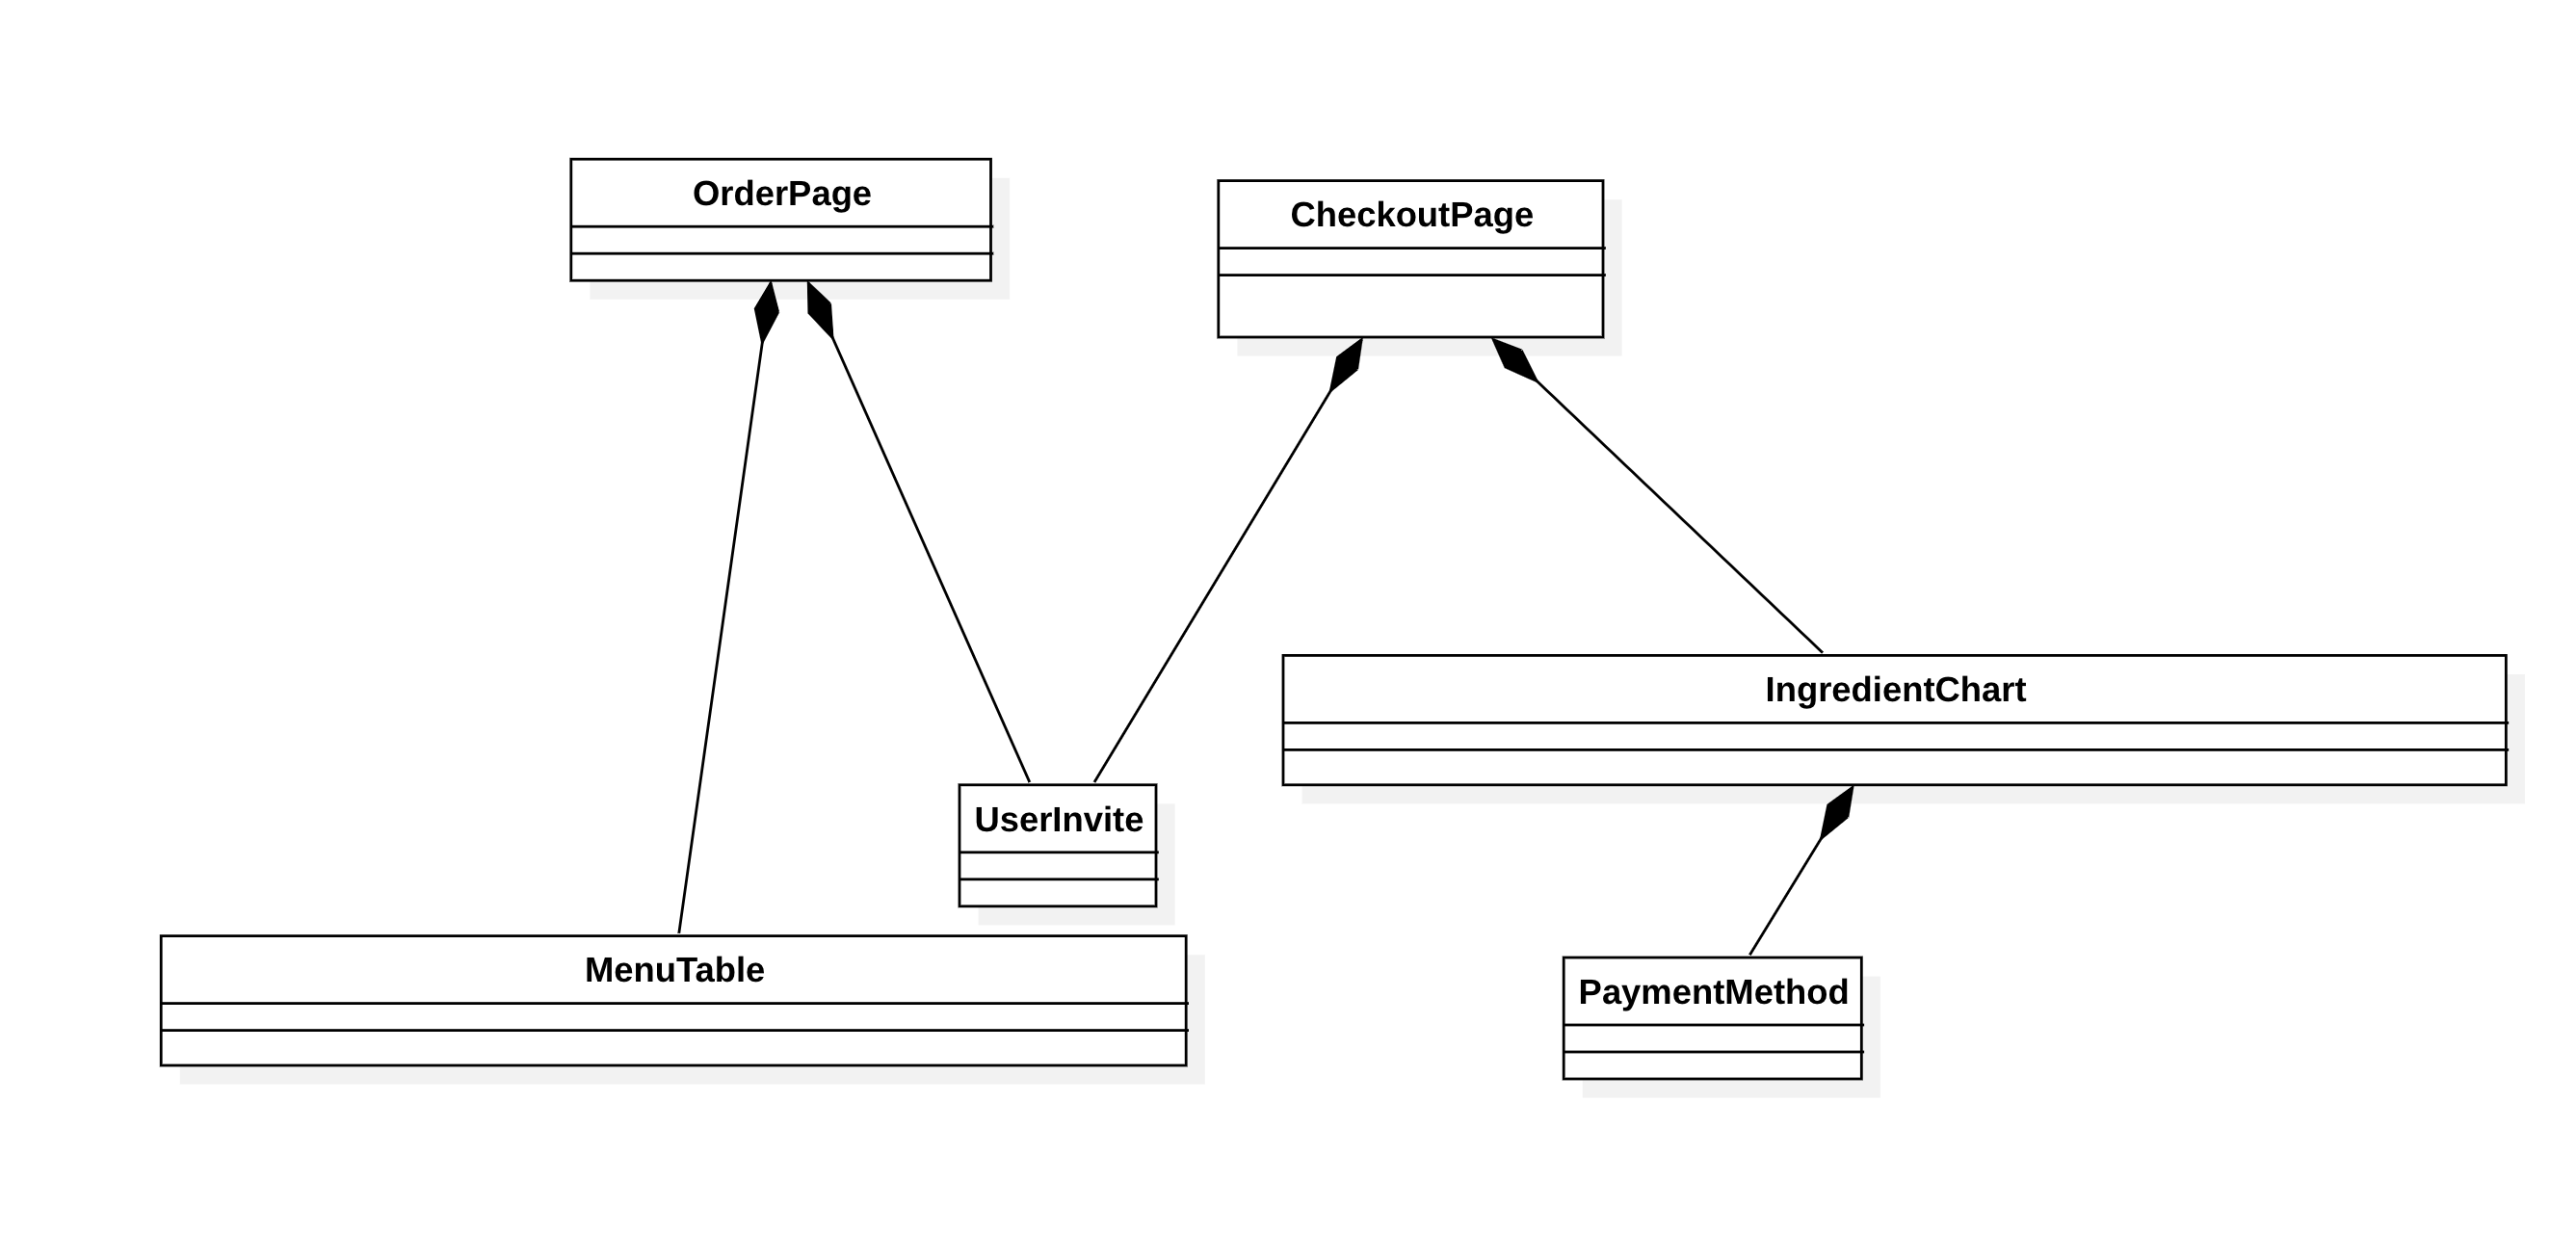
\includegraphics[width=0.8\linewidth]{images/order_page_totale}
    \caption{Diagramma UML pagina di ordinazione}
    \label{fig:UML-login}
\end{figure}
\textbf{OrderPage}
\paragraph{Descrizione} Durante la fase di $\textit{ordinazione}_G$ collaborativa, si possono vedere le informazioni del ristorante e relativa $\textit{prenotazione}_G$; questo è reso possibile dal componente OrderPage. Il componente MenuTable mostra una lista di piatti, ognuno dei quali ha a disposizione un contatore e due pulsanti per incrementare o decrementarne la quantità ordinata.\\\\
\textbf{CheckoutPage}
\paragraph{Descrizione} Una volta finito il $\textit{processo}_G$ di $\textit{ordinazione}_G$, l'utente può accedere alla pagina di checkout, la quale contiene un riepilogo degli ordini e la possibilità di togliere degli ingredienti dai piatti ordinati; alla fine della pagina è inoltre possibile scegliere come suddividere il totale del conto tra gli utenti coinvolti nella $\textit{prenotazione}_G$.
\subsubsubsection{Sign\_up}
\begin{figure}[H]
    \centering
    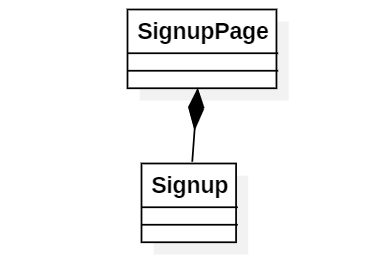
\includegraphics[width=0.45\linewidth]{images/signup.png}
    \caption{Diagramma UML pagina di sign up}
    \label{fig:UML-signup}
\end{figure}
\paragraph{Descrizione} La pagina sign up permette all'utente di registrarsi come utente base all'interno del sito, inserendo una email non presente nel $\textit{sistema}_G$, un nome, un cognome e la password. Se la registrazione avrà successo l'utente sarà reindirizzato al login.
\subsubsubsection{Sign\_up\_admin}
\begin{figure}[H]
    \centering
    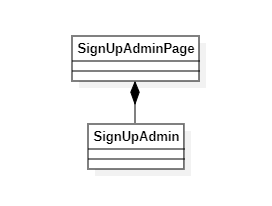
\includegraphics[width=0.45\linewidth]{images/SignUpAdmin.png}
    \caption{Diagramma UML pagina di sign up admin}
    \label{fig:UML-signupadmin}
\end{figure}
\paragraph{Descrizione} La pagina sign up admin permette all'utente di registrarsi come utente amministratore all'interno del sito, inserendo una email non presente nel $\textit{sistema}_G$, un nome, un cognome, un nome per il ristorante, una città, un indirizzo, una descrizione, degli orari di apertura e di chiusura, un numero di coperti, un numero di telefono, una email per il ristorante, una tipologia di cucina, una password e la conferma della stessa. Se la registrazione avrà successo l'utente verrà reindirizzato al login.


\subsubsubsection{User}
\begin{figure}[H]
    \centering
    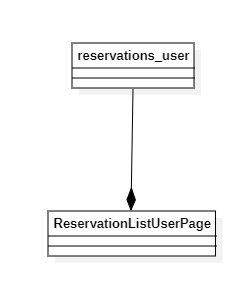
\includegraphics[width=0.3\linewidth]{images/user_reservationS_page.png}
    \caption{Diagramma UML pagina lista prenotazioni - utente base}
    \label{fig:UML-user_reservationS_page}
\end{figure}
\paragraph{Descrizione} La pagina della lista prenotazioni per l’utente riporta tutte le prenotazioni che sono state fatte nei vari ristoranti. Di ogni $\textit{prenotazione}_G$ nella lista si visualizzano: id, numero, di partecipanti, data, ora, un bottone per accedere alla singola $\textit{prenotazione}_G$ e lo stato attuale in cui si trova la $\textit{prenotazione}_G$ (in attesa di conferma, da pagare, accettata, rifiutata e completata).


\begin{figure}[H]
    \centering
    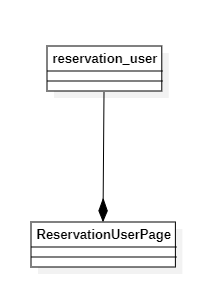
\includegraphics[width=0.3\linewidth]{images/user_reservation_page.png}
    \caption{Diagramma UML pagina prenotazione specifica - utente base}
    \label{fig:UML-user_reservationS_page}
\end{figure}
\paragraph{Descrizione} La pagina della singola $\textit{prenotazione}_G$ permette all’utente di visualizzare i dati della $\textit{prenotazione}_G$ con la possibilità di:
\begin{itemize}
    \item vedere se la $\textit{prenotazione}_G$ è stata accettata o rifiutata
    \item visualizzare i pasti ordinati se la $\textit{prenotazione}_G$ è stata accettata o completata
    \item visualizzare il costo totale e/o parziale se lo ordinazioni sono state confermate
\end{itemize}


\newpage
\subsubsection{Websocket}
Il $\textit{WebSocket}_G$ server, implementato con NestJS, è progettato per gestire la comunicazione in tempo reale tra il server e i client. Questa $\textit{architettura}_G$ permette di instaurare connessioni persistenti e bidirezionali, fornendo aggiornamenti immediati senza la necessità di interrogare continuamente il server.
\subsubsubsection{Componenti Principali}
L'$\textit{architettura}_G$ logica del $\textit{WebSocket}_G$ server si compone dei seguenti elementi principali:
\begin{itemize}
\item \textbf{Gateway $\textit{WebSocket}_G$}: La porta di ingresso principale per le connessioni $\textit{WebSocket}_G$. Questo componente gestisce la creazione, chiusura e gestione delle connessioni.
\item \textbf{Eventi e Canali}: Gestione degli eventi e dei canali attraverso cui i messaggi vengono inviati e ricevuti. Ogni canale può essere visto come un argomento specifico a cui i client possono iscriversi.
\item \textbf{Sottoscrizioni}: I client possono iscriversi a determinati eventi o canali, ricevendo notifiche ogni volta che un messaggio pertinente viene inviato.
\item \textbf{Gestione delle Connessioni}: Mantenimento dello stato delle connessioni, inclusa la gestione di eventi di connessione e disconnessione, e l'associazione dei client a specifici canali.
\item \textbf{Servizi e Controller}: Logica di business che elabora i messaggi in arrivo e genera risposte o eventi di notifica.
\end{itemize}
\begin{figure}[H]
    \centering
    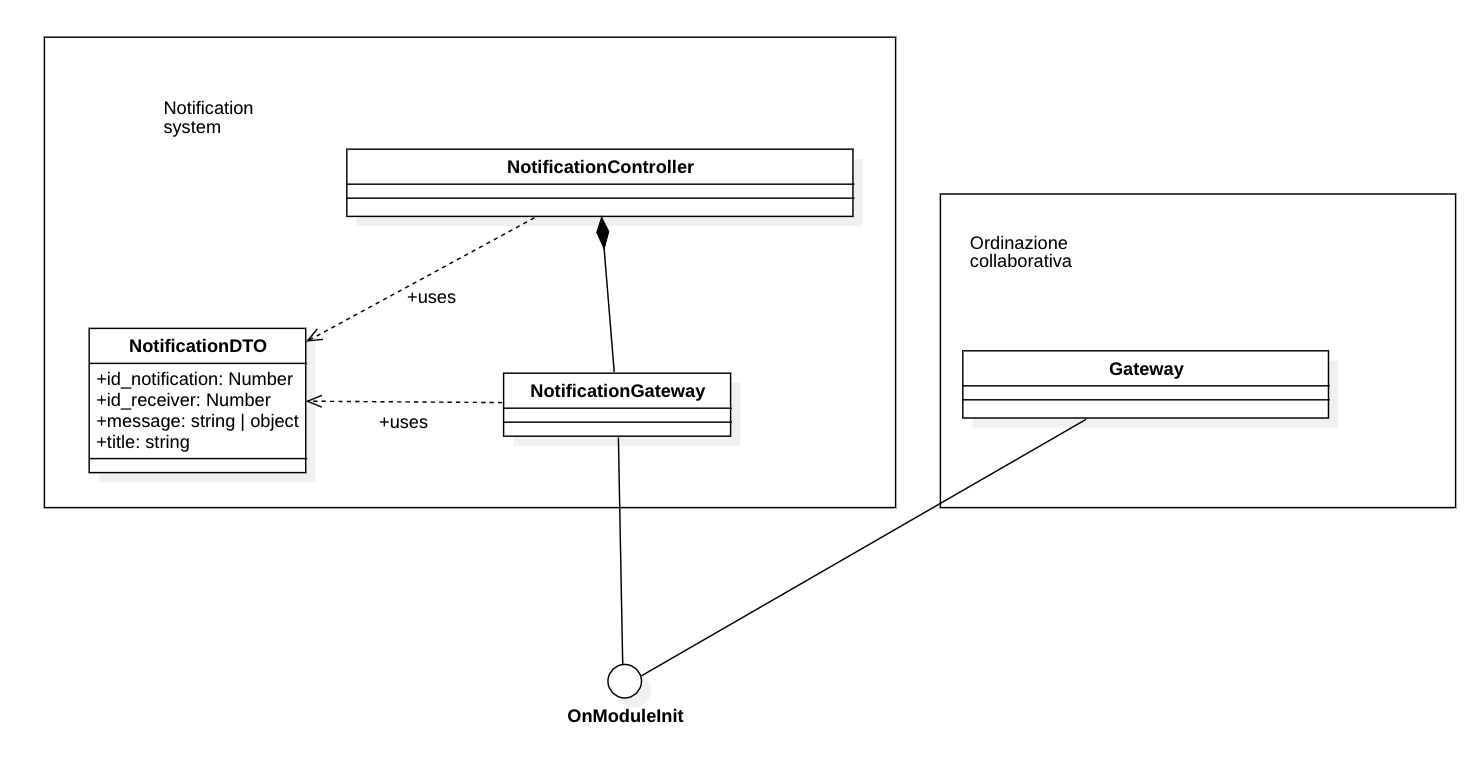
\includegraphics[width=0.95\linewidth]{images/server_websocket_noinfo}
    \caption{Diagramma UML server socket}
    \label{fig:UML-login}
\end{figure}
\begin{comment}
\subsubsubsection{Sistema di notifica}
Di seguito viene riportato il diagramma $\textit{UML}_G$ del $\textit{sistema}_G$ di notifica.
\begin{figure}[H]
    \centering
    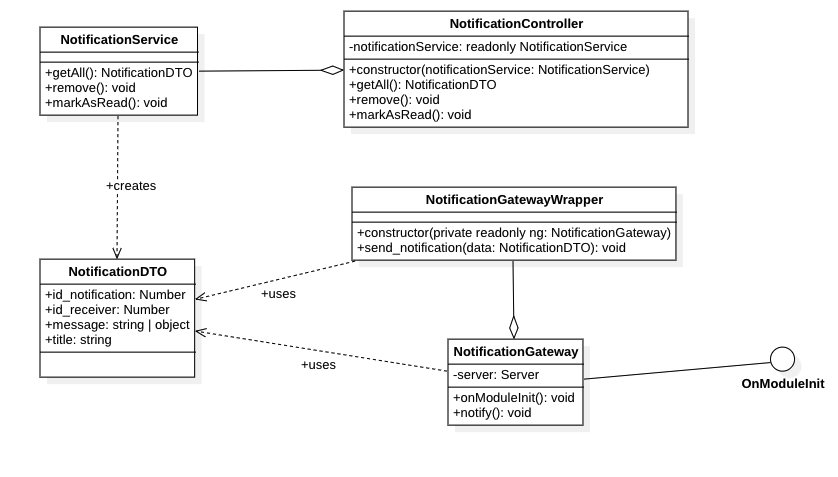
\includegraphics[width=0.7\linewidth]{images/notification_system.png}
    \caption{Diagramma UML}
    \label{fig:schemaER}
\end{figure}
\end{comment}
\newpage
\subsubsection{Database}
Il progetto utilizza PostgreSQL come $\textit{sistema}_G$ di gestione del database relazionale ($\textit{RDBMS}_G$). PostgreSQL è una scelta robusta e scalabile che offre numerose funzionalità avanzate, tra cui:

\begin{itemize}
\item \textbf{ACID Compliance}: Garantisce l'integrità dei dati attraverso le proprietà di Atomicità, Consistenza, Isolamento e Durabilità.
\item \textbf{Supporto per Transazioni}: Consente l'esecuzione sicura e affidabile delle transazioni, fondamentale per applicazioni che richiedono coerenza nei dati.
\end{itemize}
Nel contesto del nostro progetto, PostgreSQL è utilizzato per memorizzare e gestire tutti i dati dell'applicazione, inclusi gli utenti, e le transazioni in tempo reale. La configurazione del database è gestita tramite un container $\textit{Docker}_G$ dedicato, garantendo un ambiente di sviluppo e produzione coerente e facilmente replicabile.
\paragraph{Schema base di dati}
Di seguito viene riportato lo schema ER del database utilizzato
\begin{figure}[H]
    \centering
    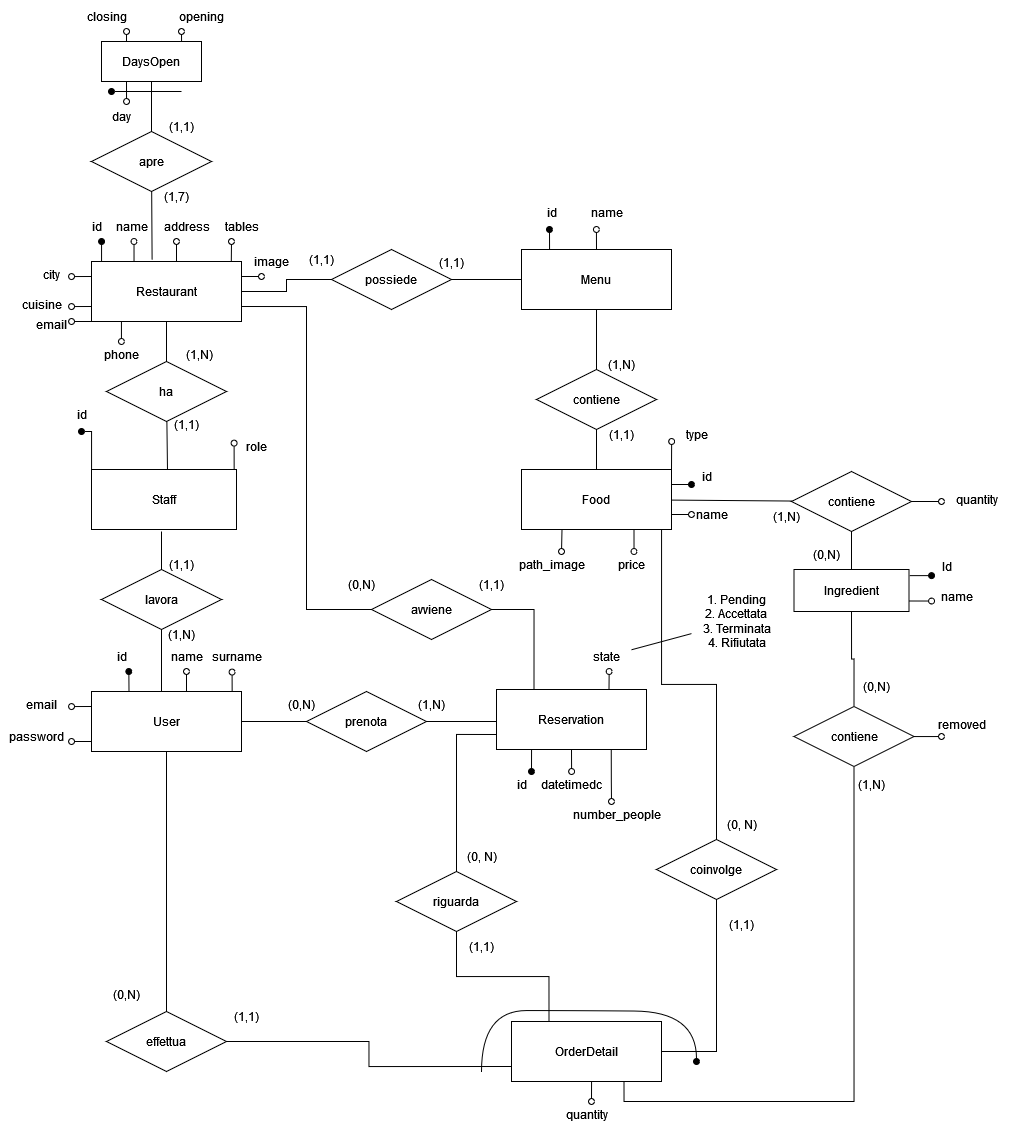
\includegraphics[width=0.85\linewidth]{images/ER.png}
    \caption{Schema ER}
    \label{fig:schemaER}
\end{figure}
\subsection{Design Pattern utilizzati}
\subsubsection{Backend}
Nel $\textit{backend}_G$ si sono utilizzati i pattern messi a disposizione dal $\textit{framework}_G$ $\textit{Nest.js}_G$.
\subsubsubsection{Dependency Injection}
Il pattern Dependency Injection ha l'obiettivo di minimizzare le dipendenze tra le classi, riducendone il grado di accoppiamento. Questo approccio migliora la modularità e la testabilità del codice.
In NestJS, il pattern Dependency Injection è implementato utilizzando il decorator @Injectable(). Grazie a questo decorator, è possibile dichiarare le classi le cui dipendenze sono gestite e iniettate dal container di iniezione delle dipendenze di NestJS.
\begin{lstlisting}[style=ES6, caption={Esempio di utilizzo della Dependency Injection con il decorator @Injectable in un servizio di autenticazione}]
@Injectable()
export class AuthenticationService {
  constructor(
    private jwtService: JwtService,
    private userService: UserService
  ) { }
}
\end{lstlisting}
Il codice mostra l'implementazione del servizio di autenticazione. Il servizio AuthenticationService è decorato con @Injectable(), il che indica che può avere dipendenze iniettate.
Il costruttore del servizio accetta due dipendenze:
\begin{itemize}
\item jwtService: un servizio fornito da NestJS per gestire la creazione e la verifica dei $\textit{JSON}_G$ Web Token ($\textit{JWT}_G$) utilizzati per l'autenticazione.
\item userService: il servizio che gestisce la logica degli user. Questo servizio viene utilizzato per recuperare informazioni sull'utente necessarie per il $\textit{processo}_G$ di autenticazione.
\end{itemize}
Questo esempio dimostra l'utilizzo del pattern Dependency Injection in NestJS, che semplifica la gestione delle dipendenze tra i vari componenti dell'applicazione. \\
\begin{lstlisting}[style=ES6, caption={Esempio di utilizzo della Dependency Injection per gestire il controller e il service}]
@Controller('authentication')
export class AuthenticationController {
  constructor(private readonly authenticationService: AuthenticationService) { }
}
\end{lstlisting}
In questo esempio, viene definito un controller AuthenticationController che gestisce le richieste relative all'autenticazione dell'applicazione. La Dependency Injection viene utilizzata per iniettare il servizio AuthenticationService all'interno del costruttore del controller.\\
Questo approccio permette al controller di accedere direttamente al servizio AuthenticationService, senza la necessità di creare istanze o gestire manualmente le dipendenze. Ciò semplifica il codice e promuove una migliore organizzazione e manutenibilità dell'applicazione.

\newpage
I vantaggi della Dependency Injection sono i seguenti:
\begin{itemize}
\item \textbf{Riduzione dell'Accoppiamento}: La DI riduce il grado di accoppiamento tra le classi, facilitando la sostituzione e la modifica dei componenti senza influenzare il resto del $\textit{sistema}_G$.
\item \textbf{Migliore Testabilità}: Le dipendenze possono essere facilmente simulate o sostituite durante i $\textit{test}_G$, rendendo il codice più $\textit{test}_G$abile.
\item \textbf{Modularità}: La DI promuove una progettazione modulare del codice, dove i componenti sono autonomi e possono essere sviluppati, testati e mantenuti indipendentemente.
\item \textbf{Manutenibilità}: Le applicazioni costruite con DI sono generalmente più facili da manutenere e scalare, poiché le dipendenze sono dichiarate e gestite dal $\textit{framework}_G$.
\item \textbf{Inversione del Controllo}: Con la DI, il controllo della creazione degli oggetti è spostato dal codice applicativo al $\textit{framework}_G$, migliorando la gestione delle dipendenze.
\end{itemize}
\subsubsubsection{Decorator pattern}

In NestJS, il pattern dei decorator viene utilizzato per definire metadati e configurare le componenti dell'applicazione. Specificando i decorator prima di definire una classe, un metodo o una proprietà, è possibile aggiungere funzionalità al codice in modo dichiarativo. Di seguito è riportata una lista dei principali decorator utilizzati nel progetto, con una spiegazione dettagliata di ciascuno:

\begin{itemize}
\item \textbf{Module}: Il decorator \texttt{@Module} viene utilizzato per definire una classe come modulo. Un modulo in NestJS è una struttura che aggrega controller, provider e dipendenze da altri moduli. Serve a organizzare il codice in unità riutilizzabili e gestibili. Esempio:
\begin{lstlisting}[style=ES6]
@Module({
  controllers: [AuthenticationController],
  providers: [AuthenticationService],
  exports: [AuthenticationService],
  imports: [ JwtModule.register(), UserModule ]
})
export class AuthenticationModule {}
\end{lstlisting}

\item \textbf{Controller}: Il decorator \texttt{@Controller} dichiara una classe come controller, il che significa che gestirà le richieste $\textit{HTTP}_G$. I metodi all'interno della classe contrassegnata come \texttt{@Controller} possono essere associati a specifiche rotte $\textit{HTTP}_G$. Esempio:
\begin{lstlisting}[style=ES6]
@Controller('authentication')
export class AuthenticationController { ... }
\end{lstlisting}

In questo caso viene passato al controller l'argomento \texttt{authentication}, in questo modo NestJS si occuperà di creare un $\textit{endpoint}_G$ raggiungibile tramite il suffisso specificato.
\item \textbf{Gestione delle richieste $\textit{HTTP}_G$}: NestJS mette a disposizione diversi decorator per gestire parametri della rotta, corpo della richiesta, e per associare una rotta a una funzione. Alcuni esempi includono \texttt{@Get}, \texttt{@Post}, \texttt{@Body}, \texttt{@Param}, \texttt{@Query}, ecc. Questi decorator aiutano a mappare gli $\textit{endpoint}_G$ $\textit{HTTP}_G$ ai metodi del controller in modo chiaro e leggibile. Esempio:

\begin{lstlisting}[style=ES6]

@Controller('authentication')
export class AuthenticationController {
  constructor(private readonly authenticationService: AuthenticationService) { }

  @Post('signin')
  @HttpCode(200)
  async signin(@Body() dto: AuthenticationDto) { ... }

  @Post('decodeToken')
  @HttpCode(200)
  async decodeToken(@Body() body: DecodeTokenDTO) { ... }
}
\end{lstlisting}

\item \textbf{Provider}: Una classe marcata come \texttt{@Injectable} può essere iniettata tramite il $\textit{sistema}_G$ di Dependency Injection di NestJS. Questo significa che può essere utilizzata come dipendenza in altre classi. Esempio:

\begin{lstlisting}[style=ES6]
@Injectable()
export class AuthenticationService {
    \\logica del servizio
}
\end{lstlisting}

\item \textbf{Validation}: NestJS permette di utilizzare dei decorator per la validazione dei dati in modo dichiarativo, tramite la libreria \texttt{class-validator}. Ad esempio, utilizzando \texttt{@IsString}, \texttt{@IsNumber}, ecc., sui campi di una classe per validare i dati in ingresso. Esempio:

\begin{lstlisting}[style=ES6]
export class AddCustomerDTO {   
    @IsJWT()
    token: string; 

    @IsNotEmpty()
    @IsNumber()
    reservation_id: number;
}
\end{lstlisting}

\end{itemize}

\newpage
Quindi i vantaggi sono: 
\begin{itemize}
\item \textbf{Leggibilità}: I decorator permettono di aggiungere metadati e comportamenti direttamente sulle classi e sui metodi, rendendo il codice più chiaro e immediato.
\item \textbf{Modularità}: Consentono di suddividere l'applicazione in moduli ben definiti, ciascuno con controller, provider e dipendenze, migliorando l'organizzazione del codice.
\item \textbf{Manutenibilità}: Grazie alla Dependency Injection gestita tramite decorator come \texttt{@Injectable}, il codice è più facilmente testabile e le dipendenze sono meglio gestite.
\item \textbf{Validazione dei dati}: I decorator di validazione permettono di definire regole direttamente sui DTO, semplificando la validazione dei dati in ingresso e riducendo il codice boilerplate.
\end{itemize}

\subsubsubsection{Repository pattern}

Il \textit{Repository Pattern} è un pattern di progettazione che facilita la separazione tra la $\textit{logica di business}_G$ e l'accesso ai dati. In NestJS, l'implementazione del \textit{Repository Pattern} permette di gestire in modo efficace le operazioni di persistenza dei dati, fornendo un'interfaccia comune per l'interazione con il database.\\
\\Il $\textit{Repository}_G$ agisce come un'interfaccia tra la $\textit{logica di business}_G$ e il $\textit{layer di persistenza}_G$. Incapsula la logica necessaria per accedere ai dati e fornisce metodi per eseguire operazioni di $\textit{CRUD}_G$ (Create, Read, Update, Delete). In questo modo, il $\textit{Repository}_G$ funge da \textit{Facade}, semplificando l'accesso ai dati e nascondendo i dettagli complessi dell'interazione con il database.

\begin{lstlisting}[style=ES6, caption={Esempio di utilizzo del $\textit{Repository}_G$ Pattern in un Service di NestJS}]
@Injectable()
export class UserService {
  constructor(
    @InjectRepository(User)
    private userRepo: Repository<User>,
    ...
  ) { }
  // logica del service
}
\end{lstlisting}
L'utilizzo del \textit{Repository Pattern} offre i seguenti vantaggi:

\begin{itemize}
    \item \textbf{Isolamento della logica di accesso ai dati}: Separando la logica di accesso ai dati dalla $\textit{logica di business}_G$, il codice diventa più organizzato e mantenibile. Le modifiche al $\textit{layer di persistenza}_G$ non influenzano direttamente la $\textit{logica di business}_G$.

    \item \textbf{Testabilità}: I $\textit{Repository}_G$ possono essere facilmente mockati durante i $\textit{test}_G$, permettendo di isolare la $\textit{logica di business}_G$ e di verificare il comportamento del codice senza dipendere da un database reale.
    
    \item \textbf{Astrazione del database}: Il $\textit{Repository}_G$ nasconde i dettagli specifici del database e fornisce un'interfaccia unificata per l'accesso ai dati. Ciò semplifica il cambio del database sottostante senza dover modificare il codice dei Service che utilizzano il $\textit{Repository}_G$.
    
\end{itemize}
In sintesi, il \textit{$\textit{Repository}_G$ Pattern} in NestJS permette di ottenere un'$\textit{architettura}_G$ pulita e modulare, migliorando l'organizzazione del codice e facilitando la testabilità e la manutenibilità dell'applicazione. Agendo come \textit{Facade}, il $\textit{Repository}_G$ semplifica l'interazione con il $\textit{layer di persistenza}_G$, nascondendo i dettagli complessi e fornendo un'interfaccia uniforme per l'accesso ai dati.

\subsubsubsection{Controller-Service pattern}
In NestJS, un $\textit{framework}_G$ per applicazioni $\textit{Node.js}_G$, si utilizza una suddivisione chiara tra la gestione delle richieste $\textit{HTTP}_G$ e la $\textit{logica di business}_G$. Questo approccio si basa sull'uso di due classi principali:

\begin{itemize}
    \item \textbf{Controller}: Il Controller è responsabile della gestione delle richieste $\textit{HTTP}_G$. Il suo compito principale è di associare le richieste ai metodi appropriati e di fungere da intermediario tra il client che effettua la richiesta e la $\textit{logica di business}_G$.
    
    \item \textbf{Service}: Il Service contiene la $\textit{logica di business}_G$ dell'applicazione ed è responsabile dell'interazione con il $\textit{layer di persistenza}_G$ dei dati. I metodi definiti in un Service possono essere chiamati sia dai Controller sia da altri Service, facilitando così la separazione delle responsabilità.
\end{itemize}
Questo pattern di separazione offre diversi vantaggi:

\begin{itemize}
    \item \textbf{Riusabilità} Separando la $\textit{logica di business}_G$ dalla gestione delle richieste $\textit{HTTP}_G$, i metodi definiti nei Service possono essere riutilizzati in diversi contesti. Ad esempio, un Service può essere utilizzato da più Controller o da altri Service, promuovendo una maggiore modularità e riusabilità del codice.
    
    \item \textbf{Testabilità}: La chiara divisione delle responsabilità facilita la scrittura di unit $\textit{test}_G$. Poiché la $\textit{logica di business}_G$ è isolata nei Service, è possibile $\textit{test}_G$are questi in modo indipendente dai Controller, assicurando che ogni componente funzioni correttamente.
    
    \item \textbf{Manutenibilità}: La separazione tra Controller e Service rende il codice più mantenibile. Eventuali modifiche alla $\textit{logica di business}_G$ nei Service non richiedono modifiche ai Controller, riducendo il rischio di introdurre errori e semplificando il $\textit{processo}_G$ di aggiornamento e miglioramento dell'applicazione.
    
\end{itemize}
In sintesi, l'uso di Controller e Service in NestJS permette di mantenere il codice organizzato, modulare e facile da testare e mantenere, migliorando la qualità e la robustezza dell'applicazione.

\newpage
\subsubsubsection{Module pattern}
Il $\textit{backend}_G$ è organizzato in moduli, ciascuno dei quali può contenere controller, servizi, provider e la connessione al database. Di seguito è riportato un esempio che mostra come specificare un controller, un service, la connessione al database e altri servizi provenienti da moduli esterni:
\begin{lstlisting}[style=ES6, caption={Esempio di modulo con controller, service, connessione al database e altri servizi da moduli esterni}]
@Module({
  controllers: [UserController],
  providers: [UserService],
  imports: [
    TypeOrmModule.forFeature([User]),
    StaffModule,
    RestaurantModule,
    DaysopenModule
  ],
  exports: [TypeOrmModule, UserService]
})
export class UserModule { }
\end{lstlisting}
L'uso dei moduli nel $\textit{backend}_G$ offre diversi vantaggi:
\begin{itemize}
  \item \textbf{Modularità}: consente di suddividere l'applicazione in componenti indipendenti, migliorando l'organizzazione del codice e la manutenibilità.
  \item \textbf{Riusabilità}: i moduli possono essere facilmente riutilizzati in diverse parti dell'applicazione o in altri progetti.
  \item \textbf{Iniezione delle dipendenze}: facilita la gestione delle dipendenze tra i vari componenti, rendendo il codice più testabile e riducendo l'accoppiamento tra le classi.
  \item \textbf{Scalabilità}: permette di scalare l'applicazione aggiungendo nuovi moduli senza influenzare il resto del $\textit{sistema}_G$.
  \item \textbf{Isolamento}: ogni modulo può essere sviluppato e testato indipendentemente, riducendo i possibili conflitti e bug.
\end{itemize}

\newpage
\subsubsection{Frontend}
Nel $\textit{frontend}_G$ si sono utilizzati i pattern messi a disposizione dal $\textit{framework}_G$ $\textit{Next.js}_G$.
\subsubsubsection{Backend for frontend}
Il Backends for Frontends (BFF) è un $\textit{design}_G$ pattern utilizzato per creare $\textit{API}_G$ specifiche per ogni tipo di client. Questo pattern prevede la creazione di uno strato di $\textit{backend}_G$ dedicato che interagisce con il $\textit{frontend}_G$, fornendo un'$\textit{API}_G$ su misura per le esigenze specifiche del client.
Di seguito vengono riportate le principali caratteristiche del BFF:
\begin{itemize}
    \item \textbf{$\textit{API}_G$ Specifiche per il Client}: Ogni tipo di client ha un proprio BFF che fornisce un'$\textit{API}_G$ ottimizzata per le sue esigenze. Questo consente di adattare l'$\textit{API}_G$ alle peculiarità del client, migliorando l'efficienza e l'esperienza utente.
    \item \textbf{Isolamento delle Logiche di Presentazione}: Il BFF si occupa della logica di presentazione, trasformando e aggregando i dati provenienti dai vari servizi $\textit{backend}_G$ per fornire al $\textit{frontend}_G$ solo ciò di cui ha bisogno in un formato conveniente.
    \item \textbf{Riduzione della Complessità del Frontend}: Spostando alcune logiche di business e aggregazione dei dati nel BFF, il $\textit{frontend}_G$ diventa più semplice e focalizzato esclusivamente sulla presentazione e interazione con l'utente.
    \item \textbf{Decoupling tra $\textit{Frontend}_G$ e Backend}: Il BFF funge da intermediario tra il frontend e i servizi $\textit{backend}_G$, consentendo una maggiore indipendenza e flessibilità nella gestione delle modifiche. Ad esempio, cambiamenti nei servizi $\textit{backend}_G$ possono essere gestiti nel BFF senza necessitare modifiche nel frontend.
    \item \textbf{Ottimizzazione delle Performance}: Il BFF può gestire la cache, la compressione dei dati e altre ottimizzazioni specifiche per migliorare le performance del client.
\end{itemize}
Di conseguenza i vantaggi sono:
\begin{itemize}
    \item \textbf{Migliore Esperienza Utente}: L'$\textit{API}_G$ personalizzata consente al $\textit{frontend}_G$ di ottenere esattamente i dati necessari in un formato ottimizzato, migliorando le performance e la reattività dell'applicazione.
    \item \textbf{Sviluppo e $\textit{Manutenzione}_G$ Separati}: Ogni BFF può essere sviluppato e mantenuto da team separati, permettendo una maggiore specializzazione e autonomia dei team di sviluppo.
    \item \textbf{Adattabilità e Flessibilità}: È possibile modificare e ottimizzare l'$\textit{API}_G$ del BFF senza influire sugli altri client o sul $\textit{backend}_G$ principale, facilitando l'adozione di nuove funzionalità e miglioramenti.
    \item \textbf{Sicurezza}: Il BFF può implementare misure di sicurezza specifiche per ogni tipo di client, migliorando la protezione dei dati e la gestione delle autorizzazioni.
\end{itemize}

\newpage
\begin{lstlisting}[style=ES6, caption={Esempio di $\textit{Backend}_G$ for Frontend}]
'use server'
...
export async function validateSignUp(prevState: any, formData: FormData) {

	// Check if email is valid
	const email = formData.get('email')?.toString()
	if (!email) {
	 return { message: 'Email is required' }
	}
	if (!String(email).includes('@')) {
	 return { message: 'Email must be valid' }
	}
    ...

    ...
	// Create the customer
	const response = await createUser({ 
		email: email, name: firstName, surname: lastName, password: password 
	});

	if (!response.ok) {
		const data = await response.json();
		if (data.message && Array.isArray(data.message))
			return { message: data.message.join(', ') };
		if (data.message)
			return { message: data.message };
		return { message: 'Registration failed' };
	}
	redirect('login?signup=success')
}
\end{lstlisting}
Il pattern $\textit{Backend}_G$ for $\textit{Frontend}_G$ è particolarmente utile in contesti in cui diversi tipi di client hanno esigenze specifiche e richiedono ottimizzazioni particolari. Aiuta a migliorare la modularità, la manutenibilità e l'efficienza dell'$\textit{architettura}_G$ complessiva, permettendo al tempo stesso un'evoluzione indipendente delle interfacce utente e dei servizi backend.
\newpage
\subsubsubsection{Compound Components}
Il pattern Compound Components è un $\textit{design}_G$ pattern utilizzato per creare componenti flessibili e riutilizzabili. Questo pattern consente ai componenti di collaborare tra loro in modo coeso, offrendo agli sviluppatori un modo potente per creare interfacce utente complesse e dinamiche.
Di seguito vengono riportate le principali caratteristiche del Compound Components pattern:
\begin{itemize}
    \item \textbf{Composizione Naturale}: I Compound Components sono costituiti da componenti più piccoli che lavorano insieme. Ad esempio, un componente di un modulo può essere composto da un <Form> principale e vari sottocomponenti come <Input>, <Label>, <Button>, ecc.
    \item \textbf{Interazione Tra Componenti}: I componenti figli comunicano con il componente genitore attraverso il contesto (Context $\textit{API}_G$) o altre forme di gestione dello stato condiviso. Questo consente ai figli di sapere del loro stato e delle loro azioni in relazione agli altri figli.
    \item \textbf{Flessibilità e Riutilizzo}: I Compound Components offrono una grande flessibilità poiché i componenti figli possono essere combinati in modi diversi, fornendo allo sviluppatore il controllo sulla struttura e il comportamento dell'interfaccia utente.
    \item \textbf{$\textit{API}_G$ Pulita}: L'$\textit{API}_G$ di un Compound Component è progettata per essere pulita e intuitiva. Gli sviluppatori possono utilizzare i componenti figli come se fossero parte di un'unica entità, senza preoccuparsi dei dettagli interni della loro implementazione.
\end{itemize}
I vantaggi del Compound Components pattern sono:
\begin{itemize}
    \item \textbf{Maggiore Modularità}: I componenti sono altamente modulari e possono essere riutilizzati in diverse parti dell'applicazione.
    \item \textbf{Manutenibilità}: La separazione delle logiche dei componenti rende il codice più facile da mantenere e testare, poiché ogni componente ha una responsabilità ben definita.
    \item \textbf{Flessibilità di Configurazione}: Gli sviluppatori possono configurare e comporre i componenti in modi diversi senza dover modificare il codice del componente principale.
\end{itemize}
\begin{lstlisting}[style=ES6, caption={Esempio di Compound Component}]
"use client";
...

export default function Header({ isLogin, isAdmin }: { isLogin: boolean, isAdmin: boolean }) {
	return (
	 <header className="bg-orange-500">
		<div className="mx-auto max-w-screen-xxl px-4 sm:px-6 lg:px-8">
	   ...
    
          ...
		</div>
	 </header>
	);
}
\end{lstlisting}
\begin{lstlisting}[style=ES6, caption={Esempio dell'uso del component}]
...
import Header from '../components/header'
...

const inter = Inter({ subsets: ['latin'] })

export const metadata: Metadata = {
  title: 'Easy Meal',
}

export default async function RootLayout({
  children,
}: {
  children: $\textit{React}_G$.$\textit{React}_G$Node
}) {
  const token = cookies().get("session")?.value;
  let isAdmin = false;
  if(token != null) 
    isAdmin = (await verifySession()).role === "admin";
  return (
    <html lang="en">
      <body className={inter.className}>
        <NotificationProvider token={token}>
          <Header isLogin={token != null} isAdmin={isAdmin}/>
          {children}
        </NotificationProvider>
      </body>
    </html>
  )
}
\end{lstlisting}
\subsubsubsection{Controlled inputs}
Il pattern dei Controlled inputs è una tecnica utilizzata nelle applicazioni $\textit{frontend}_G$ per gestire gli input degli utenti in modo prevedibile e controllato. Questo pattern si basa sull'associazione diretta dello stato di un componente con il valore degli input, fornendo così un controllo totale sugli input e sulle loro modifiche.
Di seguito vengono riportate le principali caratteristiche del Controlled inputs pattern:
\begin{itemize}
    \item \textbf{Stato Gestito}: Gli elementi di input (come <input>, <textarea>, <select>) vengono collegati allo stato del componente. Il valore dell'input è determinato dallo stato e ogni modifica all'input aggiorna lo stato.
    \item \textbf{Gestione degli Eventi}: Gli eventi di input (come onChange) vengono utilizzati per aggiornare lo stato del componente. Ogni volta che l'utente digita qualcosa nell'input, l'evento onChange viene chiamato e aggiorna lo stato con il nuovo valore.
    \item \textbf{Renders Sincronizzati}: Poiché il valore dell'input è sempre sincronizzato con lo stato del componente, ogni aggiornamento dello stato provoca un re-render del componente con il nuovo valore dell'input.
\end{itemize}
I vantaggi del Controlled inputs pattern sono:
\begin{itemize}
    \item \textbf{Prevedibilità}: Il valore degli input è sempre determinato dallo stato del componente, rendendo il comportamento degli input prevedibile e facile da gestire.
    \item \textbf{Validazione Semplificata}: Poiché tutti i valori degli input sono memorizzati nello stato, è facile eseguire la validazione in tempo reale e fornire $\textit{feedback}_G$ immediato agli utenti.
    \item \textbf{Sincronizzazione}: Il pattern garantisce che il valore visualizzato nell'input sia sempre aggiornato con l'ultimo valore dello stato, evitando discrepanze tra l'input e lo stato interno.
\end{itemize}
\begin{lstlisting}[style=ES6, caption={Esempio dell'uso del Controlled inputs pattern}]
'use client';
import { useFormState } from 'react-dom'
import { validateSignUp } from '@/src/actions/validateSignUp'

const initialState = {
  message: '',
}

export default function Signup() {
  const [state, formAction] = useFormState(validateSignUp, initialState);
  
  return (
    <>
      ...
            ...
              <form action={formAction}>
                ...

                ...
              </form>
              {state?.message && <p className="mt-4 text-center text-red-500">{state?.message}</p>}
            </div>
          </div>
        </div>
      </div>
    </>
  )
}
\end{lstlisting}
\newpage
\subsubsection{Websocket}
\subsubsubsection{Publish-Subscribe pattern}
Il \textit{Publish-Subscribe pattern} è un pattern comportamentale utilizzato per la comunicazione asincrona tra componenti di un $\textit{sistema}_G$. In questo modello, i \textit{publisher} inviano messaggi senza conoscere i destinatari, e i \textit{subscriber} ricevono messaggi senza conoscere gli mittenti. Questa separazione è resa possibile da un intermediario che gestisce la comunicazione, nel nostro caso, un $\textit{WebSocket}_G$.
\begin{lstlisting}[style=ES6, caption={Esempio di come viene definita la classe MyGateway per implementare il socket}]
import { ConnectedSocket, MessageBody, SubscribeMessage, WebSocketGateway, WebSocketServer } from "@nestjs/websockets";
import { Server, Socket } from 'socket.io'
import { Inject, OnModuleInit } from "@nestjs/common";

@WebSocketGateway({ cors: { origin: '*' } })
export class MyGateway implements OnModuleInit {
    @WebSocketServer()
    server: Server;

    async handleConnection(socket: Socket) {...}

    onModuleInit() {
    this.server.on('connection', this.handleConnection);
    }

    @SubscribeMessage('onMessage')
    async onIncrement(@MessageBody() body: any) {...}

    @SubscribeMessage('onIngredient')
    async onIngredient(@MessageBody() body: any) {...}

    @SubscribeMessage('onConfirm')
    async onConfirm(@MessageBody() body, @ConnectedSocket() client: Socket) {...}
}
\end{lstlisting}
\textbf{Dettagli dell'implementazione:}
\begin{itemize}
\item \textbf{Connessione del client:} Quando un client si connette, il metodo \texttt{handleConnection} viene chiamato per verificare il client e iscriverlo a una stanza specifica.
\item \textbf{Iscrizione agli eventi:} I client, una volta connessi, possono iscriversi a specifici eventi tramite il $\textit{WebSocket}_G$. Gli eventi gestiti in questo esempio sono \texttt{onMessage}, \texttt{onIngredient} e \texttt{onConfirm}. Quando questi eventi vengono inviati dal server, i client che si sono iscritti a tali eventi ricevono i relativi messaggi.
\item \textbf{Gestione dei messaggi:} Il $\textit{WebSocket}_G$ si occupa di distribuire i messaggi ai client iscritti e di mantenere le connessioni attive tra il server e i client.
\end{itemize}

\newpage
\textbf{Vantaggi dell'utilizzo del pattern Publish-Subscribe:}
\begin{itemize}
\item \textbf{Scalabilità:}
\begin{itemize}
\item L'implementazione non richiede un numero preciso di \textit{subscriber}, supportando facilmente un numero variabile di client connessi. Ciò consente al $\textit{sistema}_G$ di adattarsi facilmente a picchi di traffico senza compromettere le performance.
\item In termini di scalabilità orizzontale, è possibile aggiungere ulteriori server \textit{publisher} senza dover modificare l'implementazione del $\textit{sistema}_G$. Questo permette di distribuire il carico tra più server, migliorando la resilienza e la capacità di gestione delle richieste.
\end{itemize}
\item \textbf{Centralizzazione:}
\begin{itemize}
\item La presenza di un $\textit{WebSocket}_G$ come intermediario centralizzato semplifica la gestione della comunicazione tra componenti diversi. Tutti i messaggi passano attraverso il $\textit{WebSocket}_G$, rendendo più facile il monitoraggio, il debug e la gestione delle connessioni.
\item La centralizzazione facilita anche l'implementazione di funzionalità aggiuntive come la logica di distribuzione dei messaggi, la gestione delle riconnessioni e la sicurezza.
\end{itemize}
\item \textbf{Asincronicità}:
\begin{itemize}
\item Il modello asincrono consente al \textit{publisher} di inviare messaggi senza aspettare una conferma dai \textit{subscriber}. Questo significa che il \textit{publisher} può continuare a funzionare anche se non ci sono client connessi, migliorando l'efficienza del $\textit{sistema}_G$.
\item L'asincronicità riduce la latenza percepita dai client, in quanto i messaggi vengono ricevuti non appena inviati dal \textit{publisher}, senza dover attendere la disponibilità dei destinatari.
\end{itemize}
\end{itemize}

In sintesi, il \textit{Publisher-Subscriber pattern} implementato tramite $\textit{WebSocket}_G$ offre un modo flessibile, scalabile e efficiente per gestire la comunicazione tra componenti distribuiti, rendendolo ideale per applicazioni in tempo reale e sistemi con un elevato numero di client.
\newpage
\subsection{Architettura di deployment}
L'intero stack tecnologico e i layer del modello architetturale sono stati implementati ed eseguiti all'interno di un ambiente $\textit{Docker}_G$ che simula la suddivisione e la distribuzione dei servizi. Le informazioni dettagliate sulle immagini utilizzate e sulle configurazioni dell'ambiente sono disponibili nel file compose.yaml presente nella cartella root del $\textit{repository}_G$ EasyMeal del progetto.\\
Per l'ambiente di produzione, sono stati creati i seguenti container:
\begin{itemize}
    \item \textbf{postgres}: container contenente il database PostgreSQL
    \begin{itemize}
        \item \textbf{Immagine}: postgres;
        \item \textbf{Porta}: 7070;
        \item \textbf{Dipendenza}: nessuna;
        \item \textbf{Rete}: webnet.
    \end{itemize}
    \item \textbf{backend}: container contenente Nest.js
    \begin{itemize}
        \item \textbf{Build}: Dockerfile;
        \item \textbf{Porta}: 6969;
        \item \textbf{Dipendenza}: postgres;
        \item \textbf{Rete}: webnet.
    \end{itemize}
    \item \textbf{socket}: container contenente il $\textit{websocket}_G$ server
     \begin{itemize}
        \item \textbf{Build}: Dockerfile;
        \item \textbf{Porta}: 8000;
        \item \textbf{Dipendenza}: postgres;
        \item \textbf{Rete}: webnet.
    \end{itemize}
    \item \textbf{frontend}: container contenente Next.js
     \begin{itemize}
        \item \textbf{Build}: Dockerfile;
        \item \textbf{Porta}: 3000;
        \item \textbf{Dipendenza}: $\textit{backend}_G$;
        \item \textbf{Rete}: webnet.
    \end{itemize}
\end{itemize}
Nello stesso file compose.yaml si specifica i container si trovano all’interno della stessa rete webnet che utilizza il driver di rete bridge.
\begin{figure}[H]
  \centering
  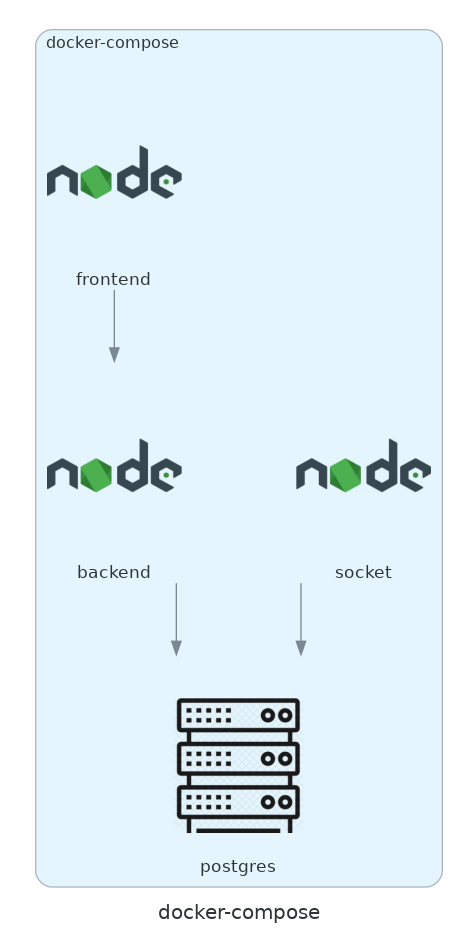
\includegraphics[width=0.4\linewidth]{images/docker-compose.png}
\caption{Archittettura di deployment del prodotto}
\end{figure}
\subsubsection{Vantaggi}
\begin{itemize}
\item \textbf{Isolamento e Consistenza}: Ogni componente è isolato in un container $\textit{Docker}_G$, garantendo che le dipendenze e le configurazioni siano coerenti tra gli ambienti di sviluppo, $\textit{test}_G$ e produzione.
\item \textbf{Scalabilità}: I servizi possono essere scalati indipendentemente a seconda delle necessità, ad esempio aumentando il numero di istanze del $\textit{backend}_G$ o del server $\textit{WebSocket}_G$ per gestire carichi di lavoro maggiori.
\item \textbf{Facilità di Manutenzione}: Con $\textit{Docker}_G$ Compose è semplice gestire e aggiornare i servizi, grazie a una singola definizione centralizzata.
\item \textbf{Portabilità}: I container $\textit{Docker}_G$ possono essere eseguiti su qualsiasi piattaforma che supporti $\textit{Docker}_G$, rendendo il $\textit{deployment}_G$ e la migrazione tra diversi ambienti molto più agevoli.
\end{itemize}
Nonostante l'uso di container per ogni componente, l'$\textit{architettura}_G$ complessiva è considerata monolitica perché tutte le parti del $\textit{sistema}_G$ (frontend, $\textit{backend}_G$ e $\textit{WebSocket}_G$ server) sono gestite come un'unica unità in quanto tutte le componenti sono strettamente collegate e dipendono l'una dall'altra per funzionare correttamente.
\newpage

% Requisiti soddisfatti
\section{Stato dei requisiti funzionali}
Di seguito vengono riportati i requisiti funzionali individuati nel documento di Analisi dei Requisiti v 2.0.0 e il loro stato in relazione all'$\textit{architettura}_G$ individuata.\\
Lo stato viene codificato con:
\begin{itemize}
    \item S: soddisfatto;
    \item NS: non soddisfatto.
\end{itemize}

\begin{longtable}{|c|c|p{12cm}|c|}
\hline
\emph{Codice} & \emph{Rilevanza} & \emph{Descrizione} & \emph{Stato} \\
\hline
\endhead
\hline

ROF 1 & Obbligatorio & L’utente deve poter selezionare un piatto dalla lista dei piatti disponibili. & S \\
\hline
RDF 2 & Desiderabile & Il $\textit{sistema}_G$ deve inviare una notifica se l'utente base sta aggiungendo un piatto che contiene elementi a cui è allergico/intollerante. & NS\\
\hline
ROF 3 & Obbligatorio & L'utente deve visualizzare i pasti con i loro ingredienti e può modificarli, togliendo o modificandone la quantità. & S\\
\hline
ROF 4 & Obbligatorio & L'utente base deve essere in grado di visualizzare il riepilogo di quanto ordinato e di confermare. & S\\
\hline
ROF 5 & Obbligatorio & Il $\textit{sistema}_G$ deve poter inviare una notifica di conferma dell'$\textit{ordinazione}_G$ collaborativa all'amministratore del ristorante & S\\
\hline
ROF 6 & Obbligatorio & L'utente deve poter inserire le informazioni (data, orario, persone) per effettuare una $\textit{prenotazione}_G$. & S\\
\hline
ROF 7 & Obbligatorio & Il $\textit{sistema}_G$ deve poter inviare una notifica all'amministratore per comunicare la richiesta di $\textit{prenotazione}_G$, che può accettare e rifiutare. & S\\
\hline
RDF 8 & Desiderabile & L'utente deve poter essere in grado di cancellare la $\textit{prenotazione}_G$. & NS\\
\hline
ROF 9 & Obbligatorio & Il $\textit{sistema}_G$ deve poter negare la $\textit{prenotazione}_G$ se il ristorante non possiede abbastanza posti o tavoli. & S\\
\hline
ROF 10 & Obbligatorio & L'utente base deve poter visualizzare una lista di ristoranti filtrata per nome oppure data, luogo, tipologia cucina. & S\\
\hline
ROF 11 & Obbligatorio & L'utente base deve poter selezionare un ristorante.  & S\\
\hline
ROF 12 & Obbligatorio & L'amministratore deve essere in grado di poter visualizzare una lista di prenotazioni in attesa. & S\\
\hline
ROF 13 & Obbligatorio & L'amministratore deve poter selezionare una specifica richiesta di $\textit{prenotazione}_G$ dalla lista visualizzata. & S\\
\hline
ROF 14& Obbligatorio & L'amministratore deve poter accettare la richiesta di $\textit{prenotazione}_G$ selezionata. & S\\
\hline
ROF 15& Obbligatorio & Il $\textit{sistema}_G$, dopo l'accettazione, aggiunge nell'area "prenotazioni" dell'utente la $\textit{prenotazione}_G$. & S\\
\hline
ROF 16& Obbligatorio & Il $\textit{sistema}_G$ deve notificare gli utenti coinvolti (nel caso di $\textit{prenotazione}_G$ collaborativa) l'accettazione della $\textit{prenotazione}_G$. & S\\
\hline
RDF 17&  Desiderabile & Il $\textit{sistema}_G$ deve fornire un'interfaccia per consentire all'amministratore di verificare la disponibilità di posti in base alle specifiche della $\textit{prenotazione}_G$ selezionata. & NS\\
\hline
RDF 18& Desiderabile &Il $\textit{sistema}_G$ deve ridurre il numero di posti disponibili in base alle specifiche della $\textit{prenotazione}_G$ dopo che questa è stata accettata. & NS\\
\hline
ROF 19& Obbligatorio &L'amministratore deve poter rifiutare la richiesta di $\textit{prenotazione}_G$ selezionata. & S\\
\hline
ROF 20& Obbligatorio &Il $\textit{sistema}_G$ deve notificare gli utenti coinvolti (nel caso di $\textit{prenotazione}_G$ collaborativa) del rifiuto della $\textit{prenotazione}_G$. & S\\
\hline
RDF 21& Desiderabile &Il $\textit{sistema}_G$ deve creare un canale di comunicazione tra l'utente e l'amministratore del ristorante quando l'utente lo richiede. & NS\\
\hline
RDF 22&  Desiderabile &L'utente e l'amministratore devono poter scambiare messaggi in modo bidirezionale tramite l'interfaccia di comunicazione. & NS\\
\hline
RDF 23&  Desiderabile &Durante la comunicazione, il $\textit{sistema}_G$ deve inviare notifiche $\textit{push}_G$ per informare l'utente e l'amministratore dei nuovi messaggi ricevuti. & NS\\
\hline
RDF 24& Desiderabile & La cancellazione della $\textit{prenotazione}_G$ può essere effettuata con al massimo un giorno di anticipo rispetto alla data della $\textit{prenotazione}_G$.  & NS\\ 
\hline
ROF 25&  Obbligatorio & Il $\textit{sistema}_G$ deve permettere di pagare il conto in base alla modalità scelta (divisione equa, divisione proporzionale) da chi ha creato la $\textit{ordinazione}_G$ collaborativa. & S\\
\hline
RDF 26& Desiderabile & L'utente base può pagare l'intero conto se nessun utente non ha ancora effettuato il pagamento. & NS\\
\hline
RDF 27& Desiderabile & L'amministratore deve poter essere in grado di modificare il menu' del proprio ristorante, aggiungendo, rimuovendo pietanze e modificando le informazioni del singolo piatto (nome, ingredienti e prezzo). & NS\\
\hline
RDF 28& Desiderabile & La modifica del menu' da parte dell'amministratore non deve causare problemi di sincronizzazione nella visualizzazione, ricerca del menu' e nell'$\textit{ordinazione}_G$ da parte dell'utente base. & NS\\
\hline
RDF 29& Desiderabile & Si deve permettere all'utente base di poter inserire un coupon prima di pagare il conto, che, se applicato, deve far ricalcolare al $\textit{sistema}_G$ il prezzo del conto. & NS\\
\hline
ROF 30& Obbligatorio & Il $\textit{sistema}_G$ deve consentire all'amministratore di visualizzare la lista delle prenotazioni effettuate per il proprio ristorante. & S\\
\hline
ROF 31& Obbligatorio & L'amministratore deve poter visualizzare i dettagli di una specifica $\textit{prenotazione}_G$. & S\\
\hline
RDF 32& Desiderabile & L'amministratore deve poter visualizzare lo stato delle ordinazioni associate alla $\textit{prenotazione}_G$. & S\\
\hline
ROF 33& Obbligatorio & Il $\textit{sistema}_G$ deve fornire all'amministratore la possibilità di visualizzare la lista totale degli ingredienti inclusi nella $\textit{prenotazione}_G$. & S\\
\hline
ROF 34& Obbligatorio & Il $\textit{sistema}_G$ deve consentire all'amministratore di visualizzare tutti gli ordini confermati per il ristorante selezionato. & S\\
\hline
RDF 35& Desiderabile & Il $\textit{sistema}_G$ deve permettere di annullare l'$\textit{ordinazione}_G$ collaborativa nel tempo utile per farlo & NS\\
\hline
RDF 36& Desiderabile &  Il $\textit{sistema}_G$ invia una notifica a tutti gli utenti associati alla $\textit{prenotazione}_G$ la cui $\textit{ordinazione}_G$ collaborativa è stata annullata & NS\\
\hline
ROF 37& Obbligatorio & Il $\textit{sistema}_G$ deve fornire un'interfaccia per consentire agli utenti non autenticati di registrarsi come utenti base. & S\\
\hline
ROF 38 & Obbligatorio & L'utente/L'amministratore deve poter inserire le sue informazioni personali durante la registrazione come nome, cognome, email, password. & S\\
\hline
ROF 39& Obbligatorio & L'utente/L'amministratore deve poter confermare di volersi registrare con le informazioni fornite prima di completare la registrazione. & S\\
\hline
ROF 40& Obbligatorio & Il $\textit{sistema}_G$ deve gestire correttamente gli errori nell'inserimento delle informazioni durante la registrazione. & S\\
\hline 
ROF 41& Obbligatorio & L'utente base e l'amministratore devono poter visualizzare il menu' del ristorante selezionato & S\\
\hline
RDF 42& Desiderabile & L'amministratore deve poter modificare le informazioni del proprio ristorante (nome, indirizzo, orari, coperti e tipologia di cucina) & NS\\
\hline
RDF 43& Desiderabile & La modifica delle informazioni del ristorante da parte dell'amministratore non deve causare problemi di sincronizzazione nella visualizzazione, ricerca del ristorante e nell'$\textit{ordinazione}_G$ da parte dell'utente base & NS\\
\hline
RDF 44& Desiderabile & L'utente autenticato deve poter visualizzare una lista con le prenotazioni passate & S\\
\hline
RDF 45& Desiderabile & L'utente autenticato deve poter rilasciare una recensione (con anche una votazione di gradimento tramite stelle) sui ristoranti nei quali ha effettuato almeno una $\textit{prenotazione}_G$ & NS\\
\hline
ROF 46& Obbligatorio & L'utente autenticato deve poter visualizzare gli ordini di un tavolo & S\\
\hline
RDF 47& Desiderabile & L'utente autenticato deve poter visualizzare le recensioni rilasciate ed eventualmente eliminarle & NS\\
\hline
RDF 48& Desiderabile & L'utente generico può visualizzare le recensioni di un ristorante e visualizzare per ognuna di essa le relative informazioni & NS\\
\hline
ROF 49& Obbligatorio & L'amministratore deve poter inserire le informazioni del ristorante di cui è amministratore & S\\
\hline
ROF 50& Obbligatorio & L'utente/L'amministratore deve poter inserire la propria email e la password durante la fase di login.  & S\\
\hline
ROF 51& Obbligatorio & Il $\textit{sistema}_G$ deve verificare che le informazioni inserite nel login corrispondano ad un account già esistente nel $\textit{sistema}_G$.  & S\\
\hline
RDF 52& Desiderabile & Il $\textit{sistema}_G$ deve predisporre un'opzione per il recupero della password  & NS\\
\hline
RDF 53& Desiderabile & L'utente non autenticato deve poter inserire la propria email durante il $\textit{processo}_G$ di recupero password.  & NS\\
\hline
RDF 54 & Desiderabile & Se l'email inserita dall'utente corrisponde ad un account nel $\textit{sistema}_G$, il $\textit{sistema}_G$ deve inviare un'email contenente un link per il recupero della password.  & NS\\
\hline
ROF 55 & Obbligatorio & Se l'email inserita dall'utente non corrisponde a un account nel $\textit{sistema}_G$, il $\textit{sistema}_G$ lo mostra a schermo.  & S\\
\hline
RDF 56 & Desiderabile & L'utente deve poter accedere a una sezione dedicata per il recupero della password tramite il link fornito nell'email di recupero password.  & NS\\
\hline
ROF 57 & Obbligatorio & Il $\textit{sistema}_G$ deve mostrare una lista di prenotazioni per l'utente base, ognuna con le seguenti informazioni:
nome del ristorante, data, ora, stato della $\textit{prenotazione}_G$ (se è ancora attiva o già completata) e numero di persone coinvolte. & S\\
\hline
RDF 58 & Desiderabile & Il $\textit{sistema}_G$ ordina la lista delle prenotazioni per data della $\textit{prenotazione}_G$.  & S\\
\hline
RDF 59 & Desiderabile & L'utente base deve poter inserire le proprie allergie/intolleranze, se presenti, durante la modifica del profilo.  & NS\\
\hline
RDF 60 & Desiderabile & L'utente autenticato e l'amministratore devono poter inserire nome, cognome, email e password nell'area di modifica delle proprie informazioni.  & NS\\
\hline
ROF 61 &  Obbligatorio & Il $\textit{sistema}_G$ deve verificare che l'email inserita dall'utente autenticato sia valida e non sia già presente nel $\textit{sistema}_G$.  & S\\
\hline
ROF 62 &  Obbligatorio & L'utente base autenticato deve poter accedere alla funzionalità di $\textit{ordinazione}_G$ di un piatto.  & S\\
\hline
ROF 63 &  Obbligatorio & Il $\textit{sistema}_G$ deve consentire all'utente di visualizzare e togliere ingredienti del piatto selezionato.  & S\\
\hline
RDF 64 & Desiderabile & L'amministratore deve poter visualizzare le recensioni del proprio ristorante. & NS\\ 
\hline
RDF 65 & Desiderabile &L'amministratore deve poter rispondere alle recensioni del proprio ristorante. & NS\\
\hline
RDF 66 & Desiderabile &L'utente deve poter visualizzare le risposte alla propria recensione. & NS\\
\hline
ROF 67 & Obbligatorio &Il $\textit{sistema}_G$ deve poter consentire di modificare l'ordine ad un utente prima della scadenza del tempo previsto, inserendo piatti, modificando ingredienti e quantità delle pietanze ordinate. & S\\
\hline
RDF 68 & Desiderabile &Il $\textit{sistema}_G$ permette di far visualizzare all'amministratore il dettaglio degli ingredienti necessari per ogni giornata. & NS\\
\hline
ROF 69 & Obbligatorio &Il $\textit{sistema}_G$ deve consentire all'utente autenticato di accedere alla funzionalità di logout. & S\\
\hline
RDF 70 & Desiderabile &Dopo che l'utente ha selezionato l'opzione di logout, il $\textit{sistema}_G$ deve richiedere una conferma esplicita dall'utente prima di procedere con la disconnessione. & NS\\ 
\hline
ROF 71 & Obbligatorio & Dopo aver terminato la sessione dell'utente, il $\textit{sistema}_G$ deve reindirizzare l'utente alla pagina di accesso o a una pagina di destinazione predefinita. & S\\
\hline
RDF 72 & Desiderabile & L'utente autenticato deve poter visualizzare le informazioni del suo profilo. & NS\\ 
\hline
RDF 73 & Desiderabile &L'amministratore deve poter visualizzare tutte le chat aperte in precedenza da altri utenti. & NS\\
\hline
RDF 74 & Desiderabile &L'amministratore deve poter rispondere ai messaggi inviati da gli utenti & NS\\
\hline
ROF 75 & Obbligatorio & Il $\textit{sistema}_G$ deve poter generare un link di invito per la $\textit{prenotazione}_G$ & S\\
\hline
RDF 76 & Desiderabile & Il $\textit{sistema}_G$ permette di far visualizzare all’amministratore in dettaglio la lista
delle prenotazioni di ogni giornata. & S\\
% Il $\textit{sistema}_G$ permette di far visualizzare all’amministratore in dettaglio la lista
% delle prenotazioni di ogni giornata.
 \hline
 ROF 77 & Obbligatorio & Il $\textit{sistema}_G$ invia una notifica all'amministratore in base agli aggiornamenti sul conto di una $\textit{prenotazione}_G$ del suo ristorante. & S\\
 \hline
\caption{Tabella dei requisiti funzionali}
\end{longtable}


% obbligatori 46
% desiderabili 31
\begin{table}[htbp]
    \centering    
\begin{spreadtab}{{tabular}{|c|c|c|c|c|}}
    \hline
    @\textbf{Rilevanza}  & @\textbf{Soddisfatti} & @\textbf{Non soddisfatti} & @\textbf{Totale} & @\textbf{Percentuale soddisfatti} \\
    \hline
    @ Obbligatori           & 40     & 0  & sum(b2:c2) &  100\%\\
    \hline
    @ Desiderabili           & 4    & 33 & sum(b3:c3) &   10.81\%\\
    \hline
\end{spreadtab}
\caption{Tabella riassuntiva dei requisiti funzionali}
\end{table}
\newpage

\end{document}